%% Преамбула TeX-файла

% 1. Стиль и язык
\documentclass[utf8x, 14pt]{G7-32} % Стиль (по умолчанию будет 14pt)

% Остальные стандартные настройки убраны в preamble.inc.tex.
\usepackage{cmap} % Улучшенный поиск русских слов в полученном pdf-файле
\usepackage[T2A]{fontenc} % Поддержка русских букв
\usepackage[utf8]{inputenc} % Кодировка utf8
\usepackage[english,russian]{babel} % Языки: русский, английский
%\usepackage{pscyr} % Нормальные шрифты
\usepackage{enumitem}

\usepackage[14pt]{extsizes}

\usepackage{caption}
\captionsetup{labelsep=endash}
\captionsetup[figure]{name={Рисунок}}

\usepackage{amsmath}

\usepackage{geometry}
\geometry{left=30mm}
\geometry{right=15mm}
\geometry{top=20mm}
\geometry{bottom=20mm}

\usepackage{titlesec}
\titleformat{\section}
	{\normalsize\bfseries}
	{\thesection}
	{1em}{}
\titlespacing*{\chapter}{0pt}{-30pt}{8pt}
\titlespacing*{\section}{\parindent}{*4}{*4}
\titlespacing*{\subsection}{\parindent}{*4}{*4}

\usepackage{setspace}
\onehalfspacing % Полуторный интервал

\frenchspacing
\usepackage{indentfirst} % Красная строка

\usepackage{titlesec}
\titleformat{\chapter}{\LARGE\bfseries}{\thechapter}{20pt}{\LARGE\bfseries}
\titleformat{\section}{\Large\bfseries}{\thesection}{20pt}{\Large\bfseries}

\usepackage{listings}
\usepackage{xcolor}

% Для листинга кода:
\lstset{ %
	language=c++,   					% выбор языка для подсветки	
	basicstyle=\small\sffamily,			% размер и начертание шрифта для подсветки кода
	numbers=left,						% где поставить нумерацию строк (слева\справа)
	%numberstyle=,					% размер шрифта для номеров строк
	stepnumber=1,						% размер шага между двумя номерами строк
	numbersep=5pt,						% как далеко отстоят номера строк от подсвечиваемого кода
	frame=single,						% рисовать рамку вокруг кода
	tabsize=4,							% размер табуляции по умолчанию равен 4 пробелам
	captionpos=t,						% позиция заголовка вверху [t] или внизу [b]
	breaklines=true,					
	breakatwhitespace=true,				% переносить строки только если есть пробел
	escapeinside={\#*}{*)},				% если нужно добавить комментарии в коде
	backgroundcolor=\color{white},
}

\usepackage{pgfplots}
\usetikzlibrary{datavisualization}
\usetikzlibrary{datavisualization.formats.functions}

\usepackage{graphicx}
\newcommand{\img}[3] {
	\begin{figure}[h!]
		\center{\includegraphics[height=#1]{inc/img/#2}}
		\caption{#3}
		\label{img:#2}
	\end{figure}
}
\newcommand{\boximg}[3] {
	\begin{figure}[h]
		\center{\fbox{\includegraphics[height=#1]{inc/img/#2}}}
		\caption{#3}
		\label{img:#2}
	\end{figure}
}

\usepackage[justification=centering]{caption} % Настройка подписей float объектов

\usepackage[unicode,pdftex]{hyperref} % Ссылки в pdf
\hypersetup{hidelinks}

\usepackage{csvsimple}



\newcommand{\code}[1]{\texttt{#1}}


% Настройки листингов.
\ifPDFTeX
% 8 Листинги

\usepackage{listings}

% Значения по умолчанию
\lstset{
  basicstyle= \footnotesize,
  breakatwhitespace=true,% разрыв строк только на whitespacce
  breaklines=true,       % переносить длинные строки
%   captionpos=b,          % подписи снизу -- вроде не надо
  inputencoding=koi8-r,
  numbers=left,          % нумерация слева
  numberstyle=\footnotesize,
  showspaces=false,      % показывать пробелы подчеркиваниями -- идиотизм 70-х годов
  showstringspaces=false,
  showtabs=false,        % и табы тоже
  stepnumber=1,
  tabsize=4,              % кому нужны табы по 8 символов?
  frame=single
}

% Стиль для псевдокода: строчки обычно короткие, поэтому размер шрифта побольше
\lstdefinestyle{pseudocode}{
  basicstyle=\small,
  keywordstyle=\color{black}\bfseries\underbar,
  language=Pseudocode,
  numberstyle=\footnotesize,
  commentstyle=\footnotesize\it
}

% Стиль для обычного кода: маленький шрифт
\lstdefinestyle{realcode}{
  basicstyle=\scriptsize,
  numberstyle=\footnotesize
}

% Стиль для коротких кусков обычного кода: средний шрифт
\lstdefinestyle{simplecode}{
  basicstyle=\footnotesize,
  numberstyle=\footnotesize
}

% Стиль для BNF
\lstdefinestyle{grammar}{
  basicstyle=\footnotesize,
  numberstyle=\footnotesize,
  stringstyle=\bfseries\ttfamily,
  language=BNF
}

% Определим свой язык для написания псевдокодов на основе Python
\lstdefinelanguage[]{Pseudocode}[]{Python}{
  morekeywords={each,empty,wait,do},% ключевые слова добавлять сюда
  morecomment=[s]{\{}{\}},% комменты {а-ля Pascal} смотрятся нагляднее
  literate=% а сюда добавлять операторы, которые хотите отображать как мат. символы
    {->}{\ensuremath{$\rightarrow$}~}2%
    {<-}{\ensuremath{$\leftarrow$}~}2%
    {:=}{\ensuremath{$\leftarrow$}~}2%
    {<--}{\ensuremath{$\Longleftarrow$}~}2%
}[keywords,comments]

% Свой язык для задания грамматик в BNF
\lstdefinelanguage[]{BNF}[]{}{
  morekeywords={},
  morecomment=[s]{@}{@},
  morestring=[b]",%
  literate=%
    {->}{\ensuremath{$\rightarrow$}~}2%
    {*}{\ensuremath{$^*$}~}2%
    {+}{\ensuremath{$^+$}~}2%
    {|}{\ensuremath{$|$}~}2%
}[keywords,comments,strings]

% Подписи к листингам на русском языке.
\renewcommand\lstlistingname{Листинг}
\renewcommand\lstlistlistingname{Листинги}

\else
\usepackage{local-minted}
\fi

% Полезные макросы листингов.
% Любимые команды
\newcommand{\Code}[1]{\textbf{#1}}


\begin{document}

\frontmatter % выключает нумерацию ВСЕГО; здесь начинаются ненумерованные главы: реферат, введение, глоссарий, сокращения и прочее.

% Стиль титульного листа и заголовки
% 
\begin{titlepage}
	\newgeometry{pdftex, left=2cm, right=2cm, top=2.5cm, bottom=2.5cm}
	\fontsize{12pt}{12pt}\selectfont
	\noindent \begin{minipage}{0.15\textwidth}
		
\includegraphics[width=\linewidth]{inc/img/b_logo.jpg}
	\end{minipage}
	\noindent\begin{minipage}{0.9\textwidth}\centering
		\textbf{Министерство науки и высшего образования Российской Федерации}\\
		\textbf{Федеральное государственное бюджетное образовательное учреждение высшего образования}\\
		\textbf{«Московский государственный технический университет имени Н.Э.~Баумана}\\
		\textbf{(национальный исследовательский университет)»}\\
		\textbf{(МГТУ им. Н.Э.~Баумана)}
	\end{minipage}
	
	\noindent\rule{18cm}{3pt}
	\newline\newline
	\noindent ФАКУЛЬТЕТ $\underline{\text{«Информатика и системы управления»~~~~~~~~~~~~~~~~~~~~~~~~~~~~~~~~~~~~~~~~~~~~~~~~~~~~~~~}}$ \newline\newline
	\noindent КАФЕДРА $\underline{\text{«Программное обеспечение ЭВМ и информационные технологии»(ИУ7)~~~~~~~~~~~~~~}}$\newline\newline
	\noindent НАПРАВЛЕНИЕ ПОДГОТОВКИ $\underline{\text{09.03.04 «Программная инженерия»~~~~~~~~~~~~~~~~~~~~~~~~~~~~~~~ }}$\newline\newline\newline\newline\newline\newline\newline
	
	
	\begin{center}
		\Large\textbf{О Т Ч Е Т}\newline
		\Large\textbf {по лабораторной работе № 4}\newline
	\end{center}
	
	\noindent\textbf{Название} $\underline{\text{~~Методология разработки и верификации ускорителей вычислений ~~~~~~~~~~~~~~~~~}}$\newline\newline
	$\underline{\text{ на платформе Xilinx Alveo~~~~~~~~~~~~~~~~~~~~~~~~~~~~~~~~~~~~~~~~~~~~~~~~~~~~~~~~~~~~~~~~~~~~~~~~~~~~~~~~~~~~~~~~~}}$\newline\newline
	\noindent\textbf{Дисциплина} $\underline{\text{~Архитектура элекронно-вычислительных машин~~~~~~~~~~~~~~~~~~~~~~~~~~~~~~~~~~~~~~~}}$\newline\newline\newline
	\newline
	
	\noindent\begin{tabular}{lcc}
		Студент: ~~~~~~~~~~~~~~~~~~~~~~~~~~~~~~~~~~~~~~~~~~~~~~~~~~~~~~~~ & $\underline{\text{~~~~~~~~~~~~~~~~}}$ & $\underline{\text{~~Козлова И. В.~~}}$       \\
		& \footnotesize подпись, дата           & \footnotesize Фамилия, И.О.                \\
		%& &  \\
		Преподаватель:                                                    & $\underline{\text{~~~~~~~~~~~~~~~~}}$ & $\underline{\text{~~~~Попов А. Ю.~~~}}$   \\
		& \footnotesize подпись, дата           & \footnotesize Фамилия, И. О.               \\
		
	\end{tabular}

	\begin{center}
		\vfill
		Москва~---~\the\year
		~г.
	\end{center}
	\restoregeometry
\end{titlepage}



\setcounter{page}{2}

\tableofcontents

\StructuredChapter{Введение}

Ускорителями вычислений принято называть специальные аппаратные устройства, способные выполнять ограниченный ряд задач с большей параллельностью и за меньшее время в сравнении с универсальными микропроцессорными ЭВМ . Как правило, ускоритель представляет собой структуру, включающую большое количество примитивных микропроцессорных устройств, объединенных шинами связей.

В настоящее время применение ускорителей вычислений охватывает ряд важных областей: финансовые вычисления, ускорение запросов к базам данных, машинное обучение, видео-аналитика. В ряде случаев удается достичь ускорения более чем в 90 раз по сравнению с универсальными ЭВМ, построенными на микропроцессорах Intel x86.

\textbf{Цель работы}: изучение архитектуры гетерогенных вычислительных систем и технологии разработки ускорителей вычислений на базе ПЛИС фирмы Xilinx.
Для достижения данной цели необходимо выполнить следующие задачи:
\begin{itemize}
\item изучить основные сведения о платформе Xilinx Alveo U200;
\item разработать RTL описание ускорителя вычислений по индивидуальному варианту;
\item выполнить генерацию ядра ускорителя;
\item выполнить синтез и сборку бинарного модуля ускорителя;
\item разработать и отладить тестирующее программное обеспечение на серверной хост-платформе;
\item провести тесты работы ускорителя вычислений.
\end{itemize}

Все задания выполняются в соответствии с вариантом №4.



\mainmatter % это включает нумерацию глав и секций в документе ниже

\setcounter{chapter}{0}

\chapter{Изучение работы шины AXI}

В данном разделе приведены диаграммы, иллюстрирующие процесс рукопожатия и пакетного чтения.

\section{Симуляция программы общего варианта}
Каналы позволяют сформировать конвейерные транзакции чтения и записи. Последовательность событий транзакции чтения можно представить следующим образом: ARVALID -> ARREADY -> RVALID -> RREADY. На рисунке \ref{readTrans} приведена транзакция чтения данных вектора на шине AXI4 MM из DDR памяти.

\begin{figure}[h!p]
	\centering
	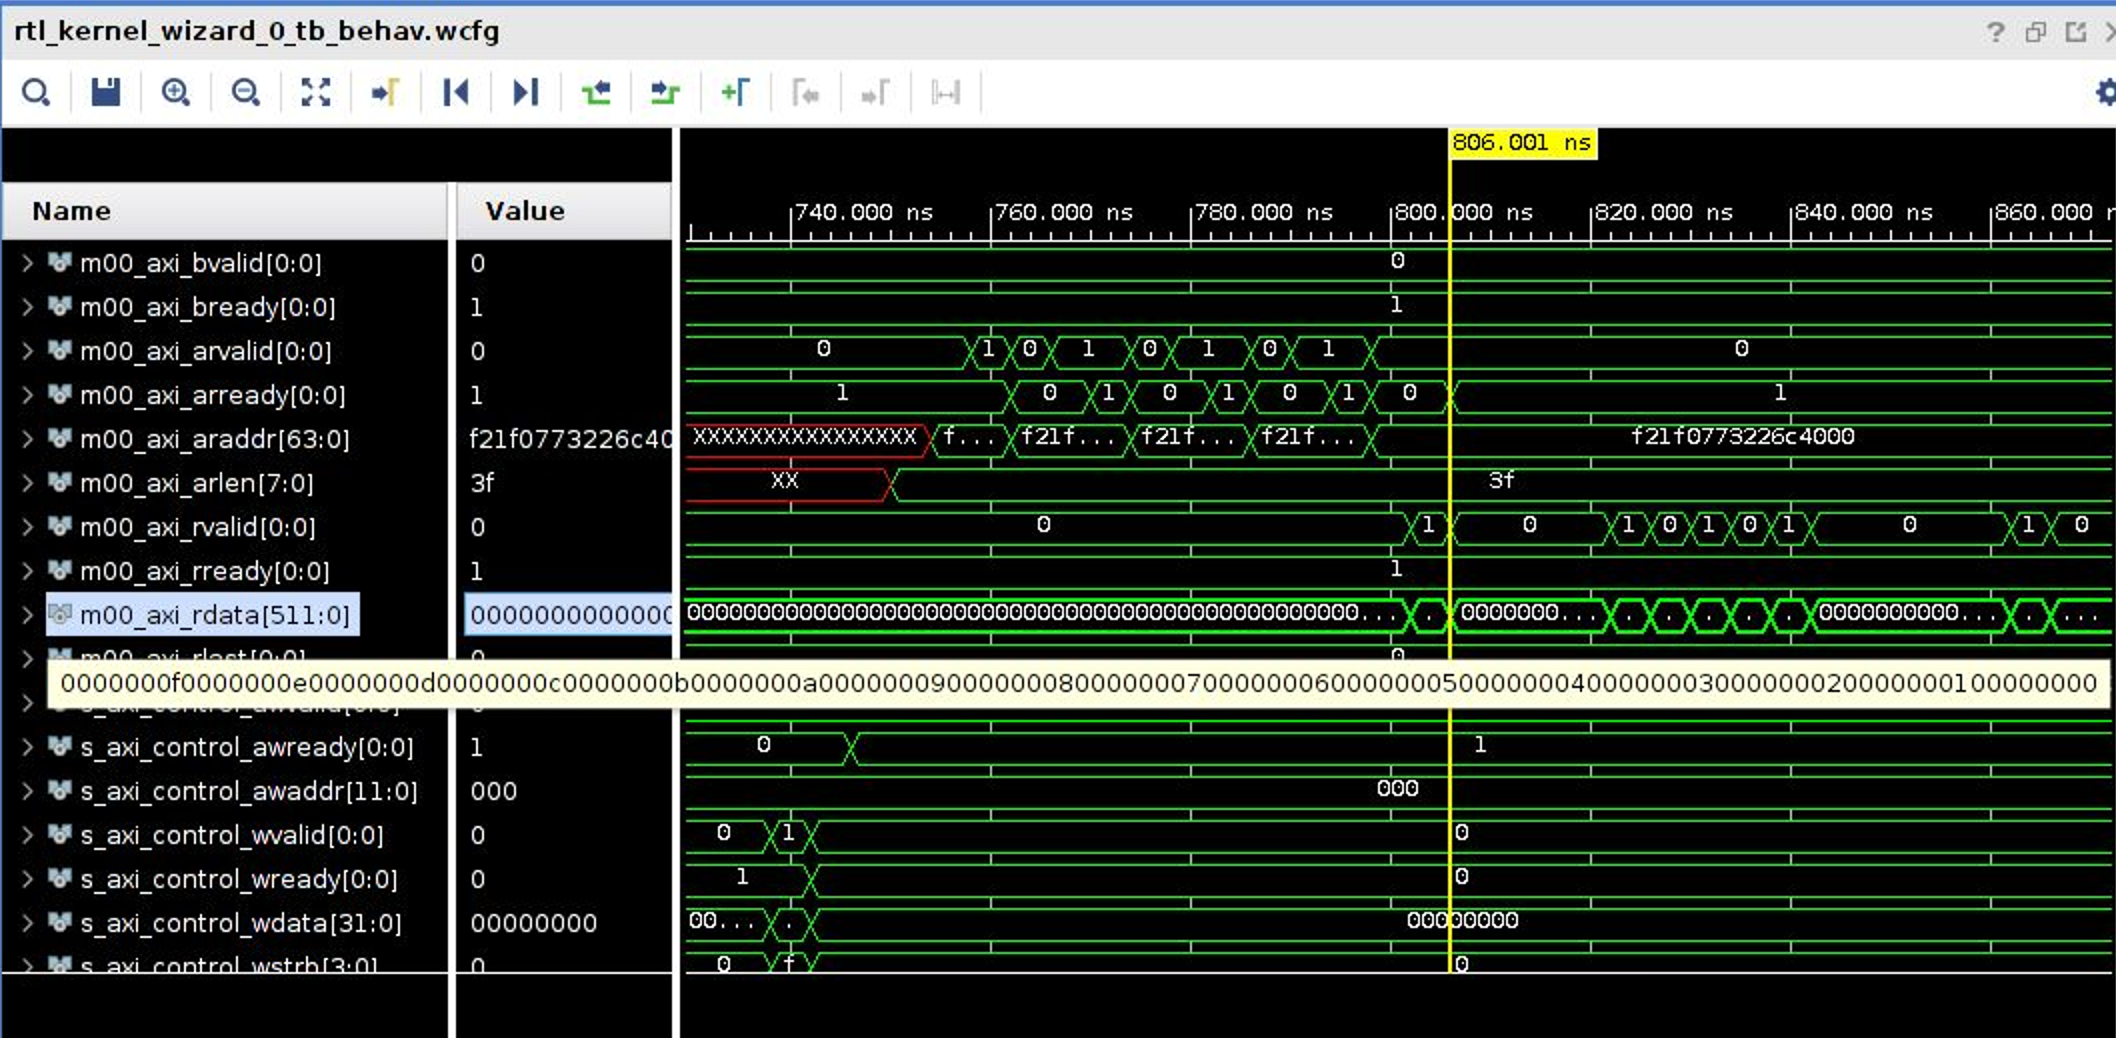
\includegraphics[width = \linewidth]{inc/read.png}
	\caption{Транзакция чтения данных вектора на шине AXI4 MM из DDR памяти}
	\label{readTrans}
\end{figure}
\newpage
Последовательность событий транзакции записи: AWVALID→ AWREADY → WVALID → WREADY → BVALID → BREADY. На рисунке \ref{writeTrans} приведена транзакция записи результата инкремента данных на шине AXI4 MM.

\begin{figure}[h!p]
	\centering
	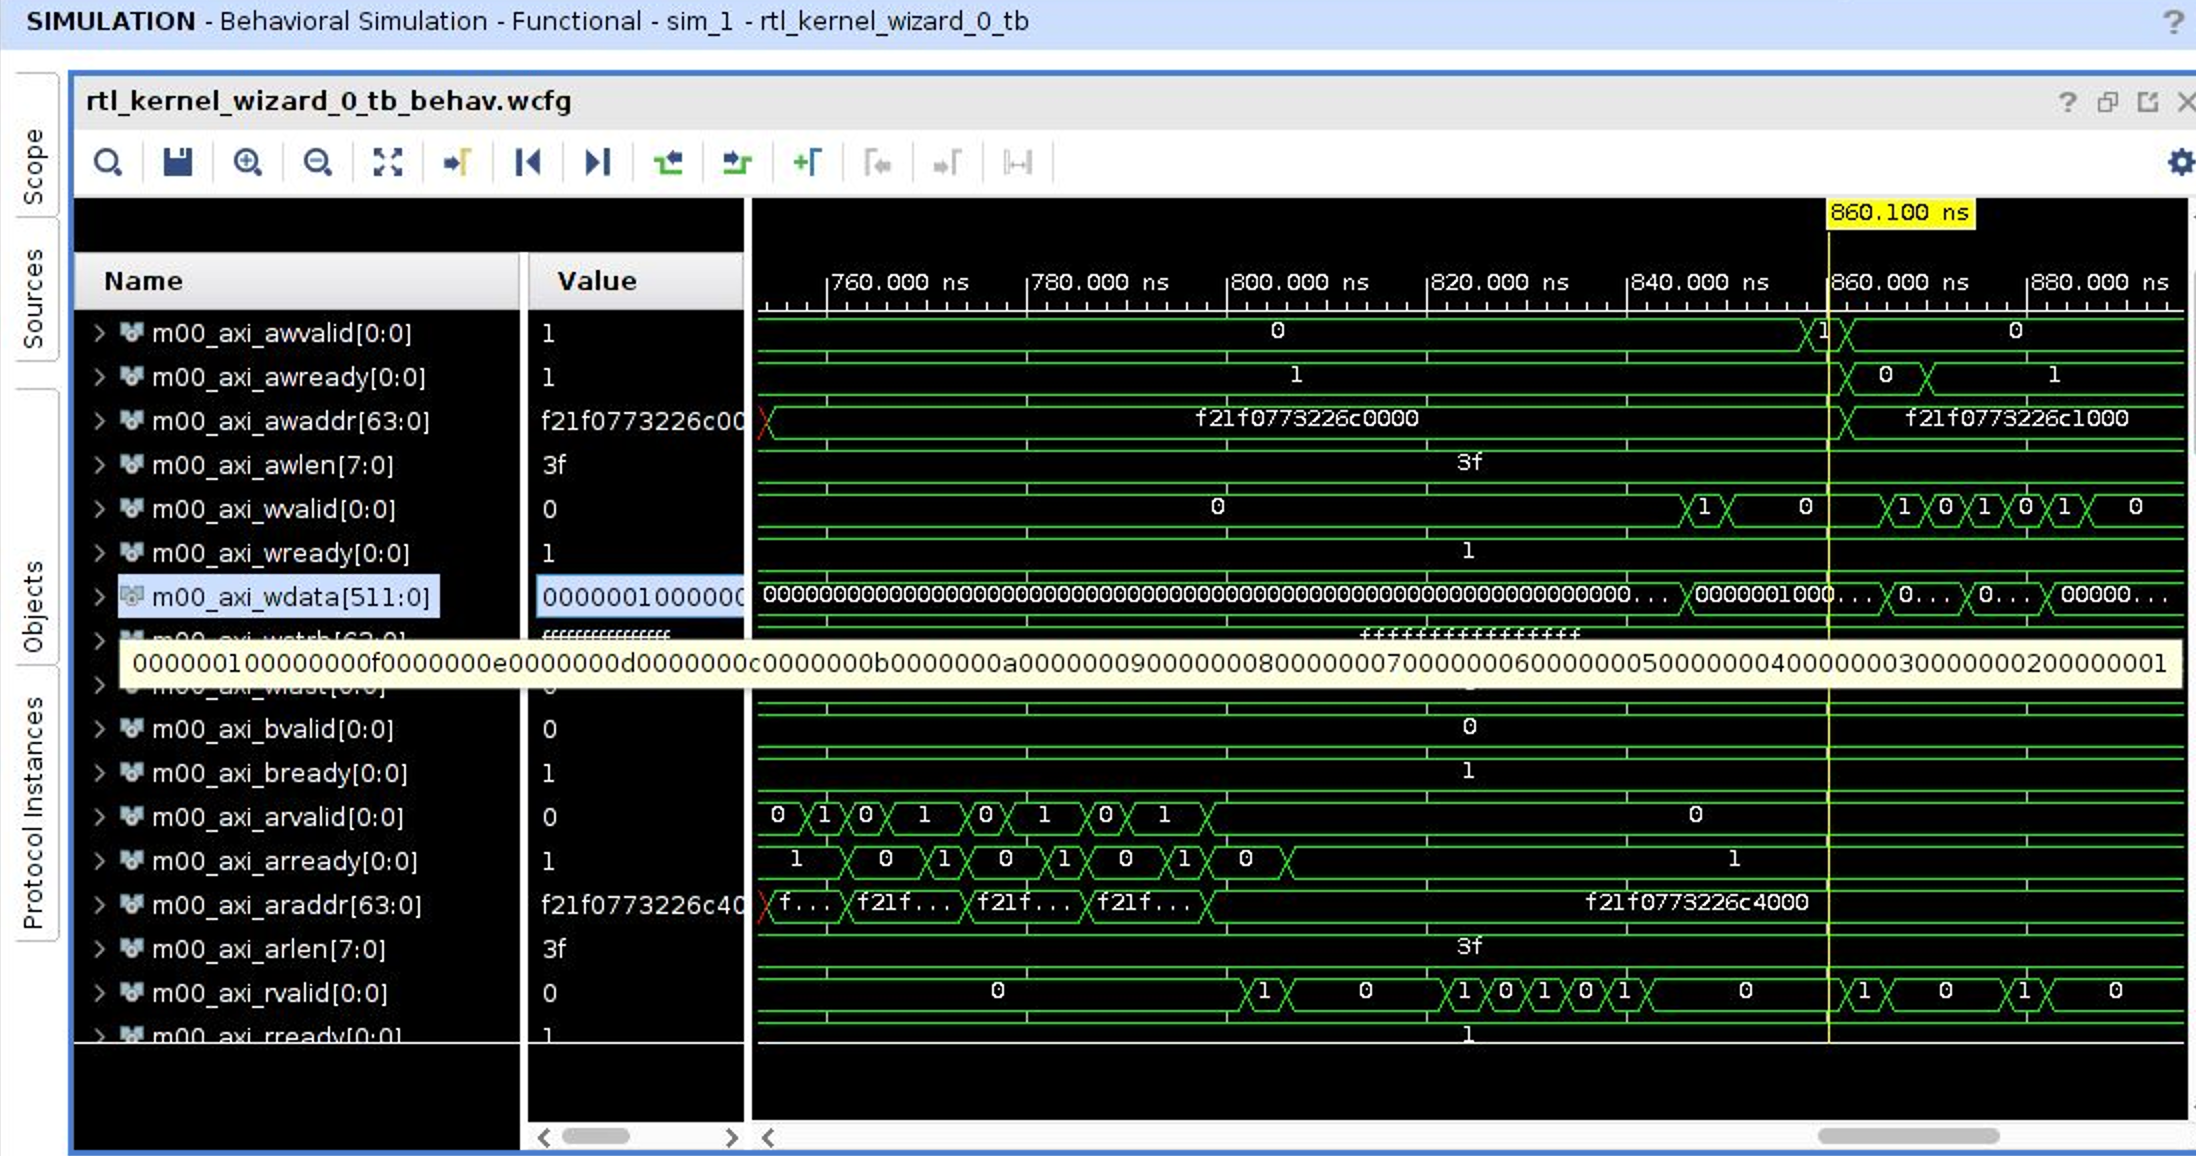
\includegraphics[width = \linewidth]{inc/write.png}
	\caption{Транзакция записи результата инкремента данных на шине AXI4 MM}
	\label{writeTrans}
\end{figure}

На рисунке \ref{incTr} приведен инкремент данных. 

\begin{figure}[h!p]
	\centering
	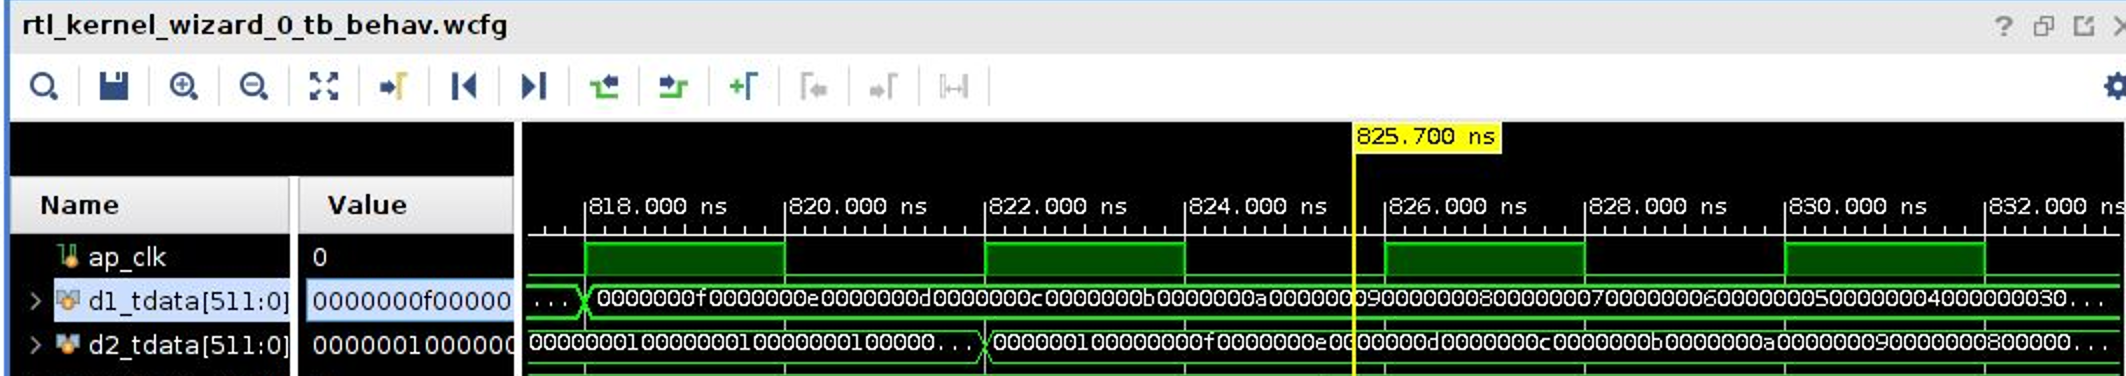
\includegraphics[width = \linewidth]{inc/inc.png}
	\caption{Инкремент данных в модуле}
	\label{incTr}
\end{figure}
\newpage
\section{Симуляция программы индивидуального варианта}
Теперь изменим модуль так, чтобы ускоритель выполнял функцию из индивидуального задания. Сделанные изменения отражены в листинге \ref{func}.
\begin{lstlisting}[label=func,caption=Модифицированная функция]
always @( posedge s_axis_aclk ) begin
    for (i=0; i<LP_NUM_LOOPS; i=i+1) begin
        d2_tdata[i*C_ADDER_BIT_WIDTH+:C_ADDER_BIT_WIDTH] <= (d1_tdata[C_ADDER_BIT_WIDTH*i+:C_ADDER_BIT_WIDTH] > 61680 ? d1_tdata[C_ADDER_BIT_WIDTH*i+:C_ADDER_BIT_WIDTH] : 61680) + 1;
    end
end
\end{lstlisting}

На рисунке \ref{readTransVar} приведена транзакция чтения данных вектора на шине AXI4 MM из DDR памяти.

\begin{figure}[h!p]
	\centering
	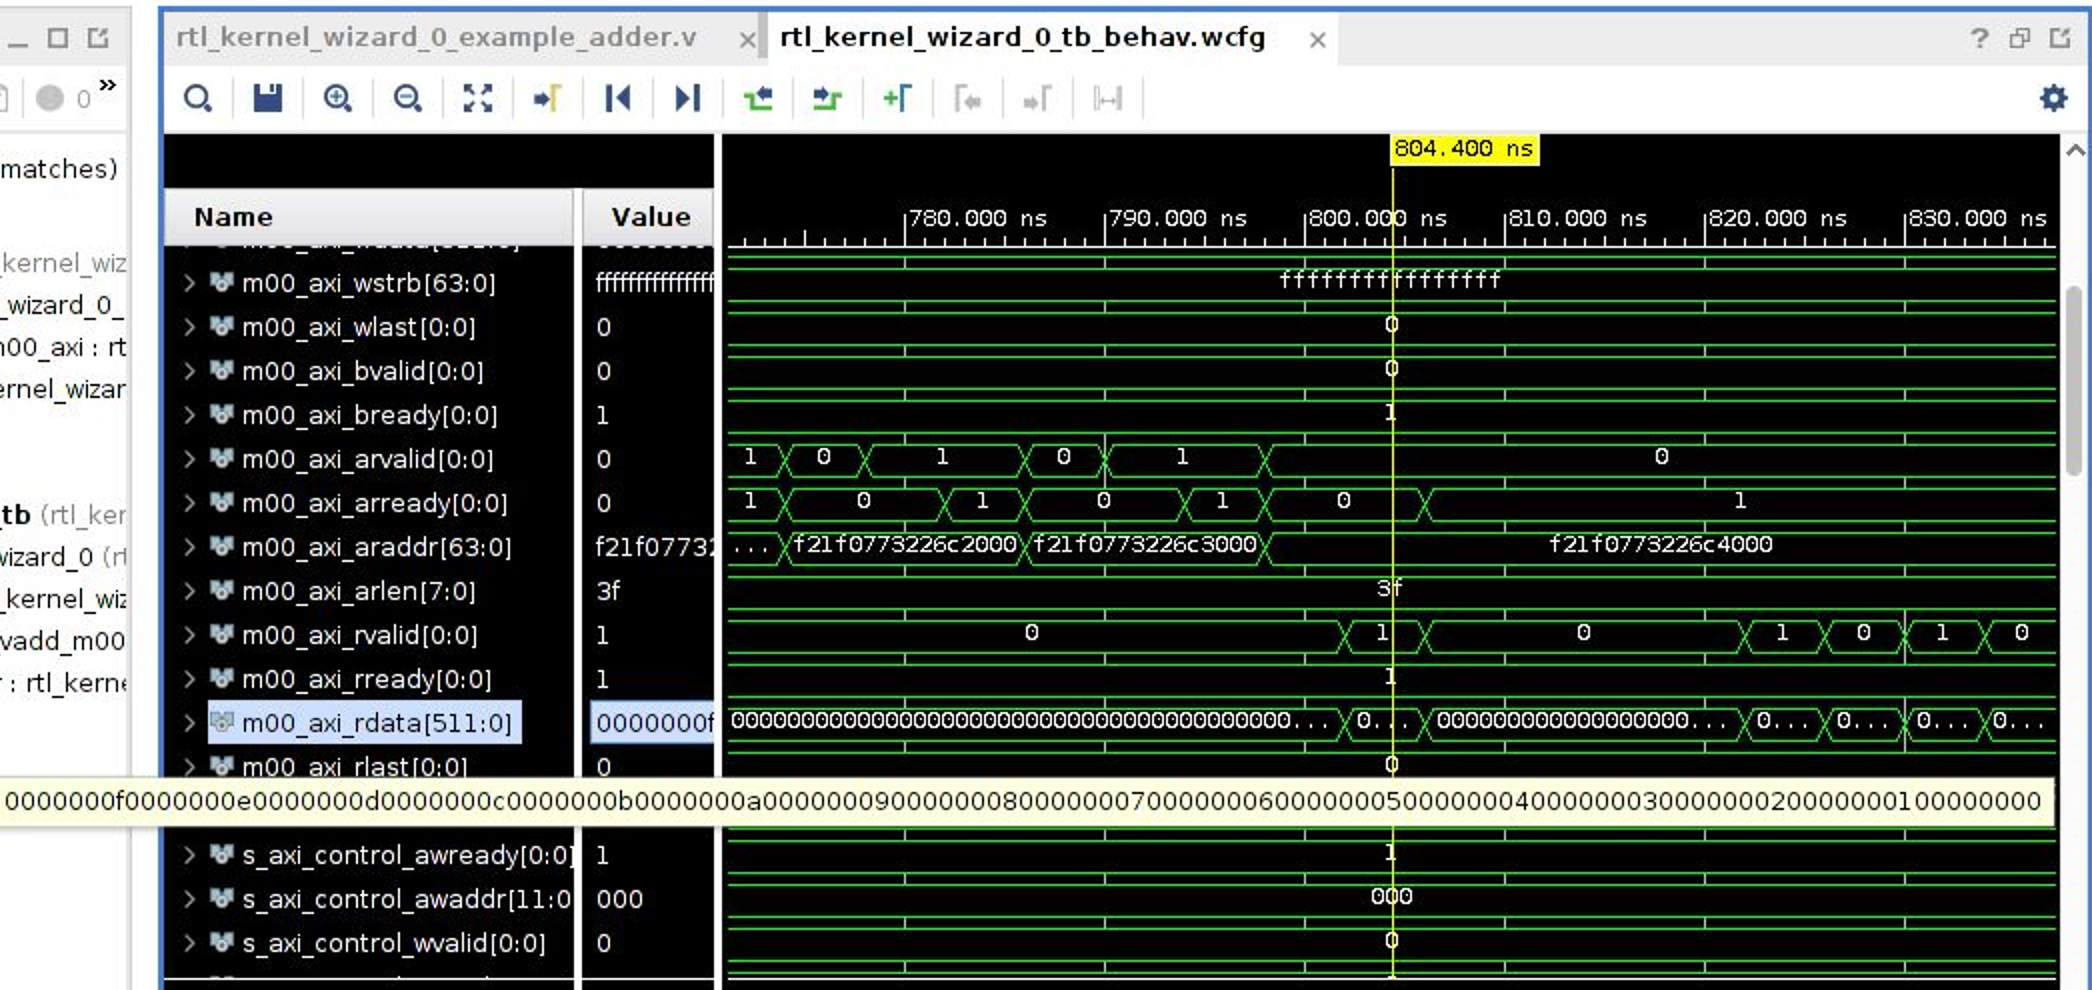
\includegraphics[width = \linewidth]{inc/read_var.png}
	\caption{Транзакция чтения данных вектора на шине AXI4 MM из DDR памяти}
	\label{readTransVar}
\end{figure}
\newpage
На рисунке \ref{writeTransVar} приведена транзакция записи результата инкремента данных на шине AXI4 MM.

\begin{figure}[h!p]
	\centering
	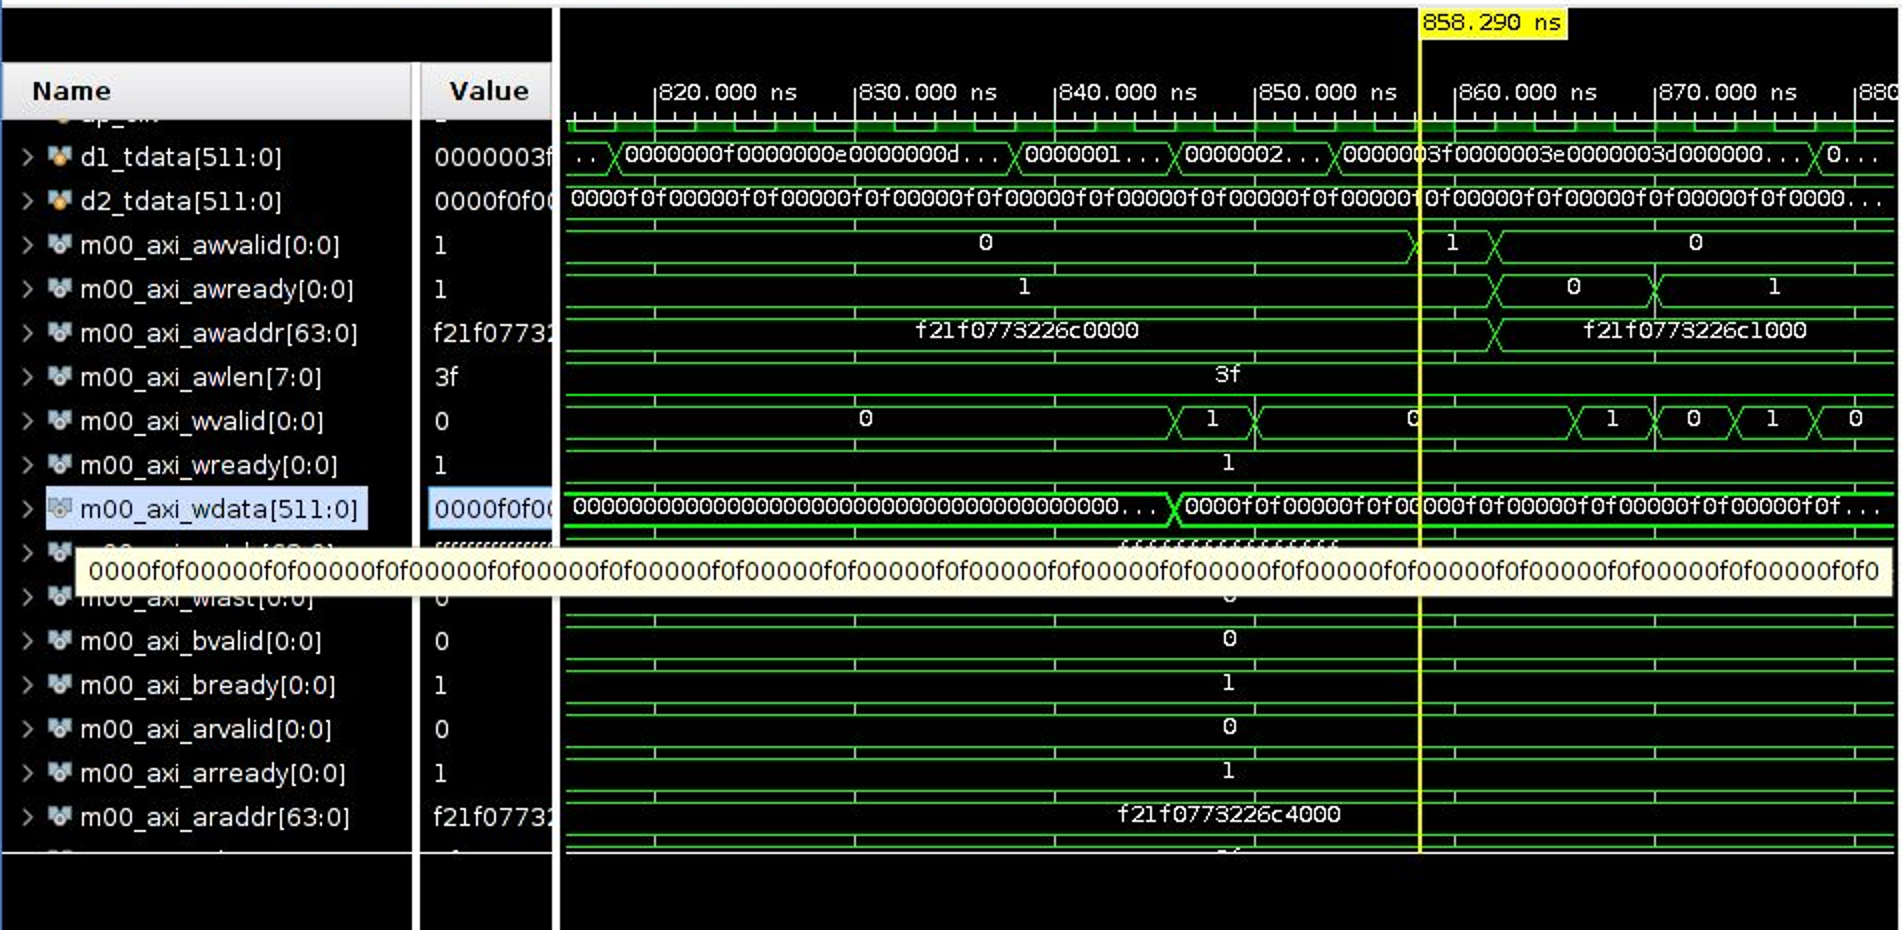
\includegraphics[width = \linewidth]{inc/write_var.png}
	\caption{Транзакция записи результата инкремента данных на шине AXI4 MM}
	\label{writeTransVar}
\end{figure}

На рисунке \ref{incTrVar} приведен инкремент данных. 

\begin{figure}[h!p]
	\centering
	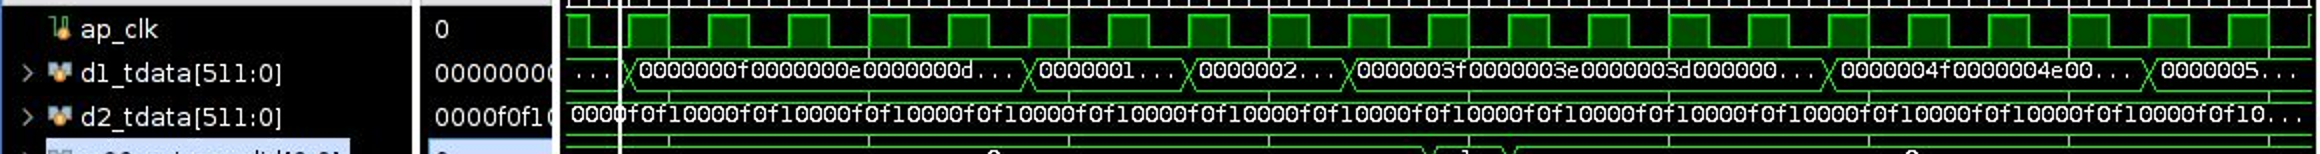
\includegraphics[width = \linewidth]{inc/inc_var.png}
	\caption{Инкремент данных в модуле}
	\label{incTrVar}
\end{figure}

\chapter{Сборка проекта}
В листинге \ref{config} приведено содержимое конфигурационного файла. В соответствии с вариантом требовалось использовать регионы SLR2, DDR[3].
\begin{lstlisting}[label=config,caption=Содержимое файла конфигурации.]
[connectivity]
nk=rtl_kernel_wizard_0:1:vinc0

slr=vinc0:SLR2

sp=vinc0.m00_axi:DDR[3]
sp=vinc0.m00_axi:PLRAM[0]

[vivado]
prop=run.impl_1.STEPS.OPT_DESIGN.ARGS.DIRECTIVE=Explore
prop=run.impl_1.STEPS.PLACE_DESIGN.ARGS.DIRECTIVE=Explore
prop=run.impl_1.STEPS.PHYS_OPT_DESIGN.IS_ENABLED=true
prop=run.impl_1.STEPS.PHYS_OPT_DESIGN.ARGS.DIRECTIVE=AggressiveExplore
prop=run.impl_1.STEPS.ROUTE_DESIGN.ARGS.DIRECTIVE=Explore
\end{lstlisting}

Содержимое файлов v++*.log и *.xclbin.info. приведено в приложениях Б и В.

\chapter{Запуск программного обеспечения на хост-системе}

В листинге \ref{code:hostexample1} приведена измененная части файла host\_example.cpp. Всё содержимое файла приведено в приложении A.

\begin{lstlisting}[label=code:hostexample1, caption=Модуль host\_example.cpp]
// Check Results

for (cl_uint i = 0; i < number_of_words; i++) {
        unsigned res = (h_data[i] > 61680 ? h_data[i] : 61680) + 1;
        if (res != h_axi00_ptr0_output[i]) {
            printf("ERROR in rtl_kernel_wizard_0::m00_axi - array index %d (host addr 0x%03x) - input=%d (0x%x), output=%d (0x%x)\n", i, i*4, h_data[i], h_data[i], h_axi00_ptr0_output[i], h_axi00_ptr0_output[i]);
            check_status = 1;
        }
      //  printf("i=%d, input=%d, output=%d\n", i,  h_axi00_ptr0_input[i], h_axi00_ptr0_output[i]);
    }
\end{lstlisting}

Для отладки и проверки работоспособности была использована утилита xgdb. На рисунке \ref{img:test} приведены результаты тестирования.

\begin{figure}[h!p]
	\centering
	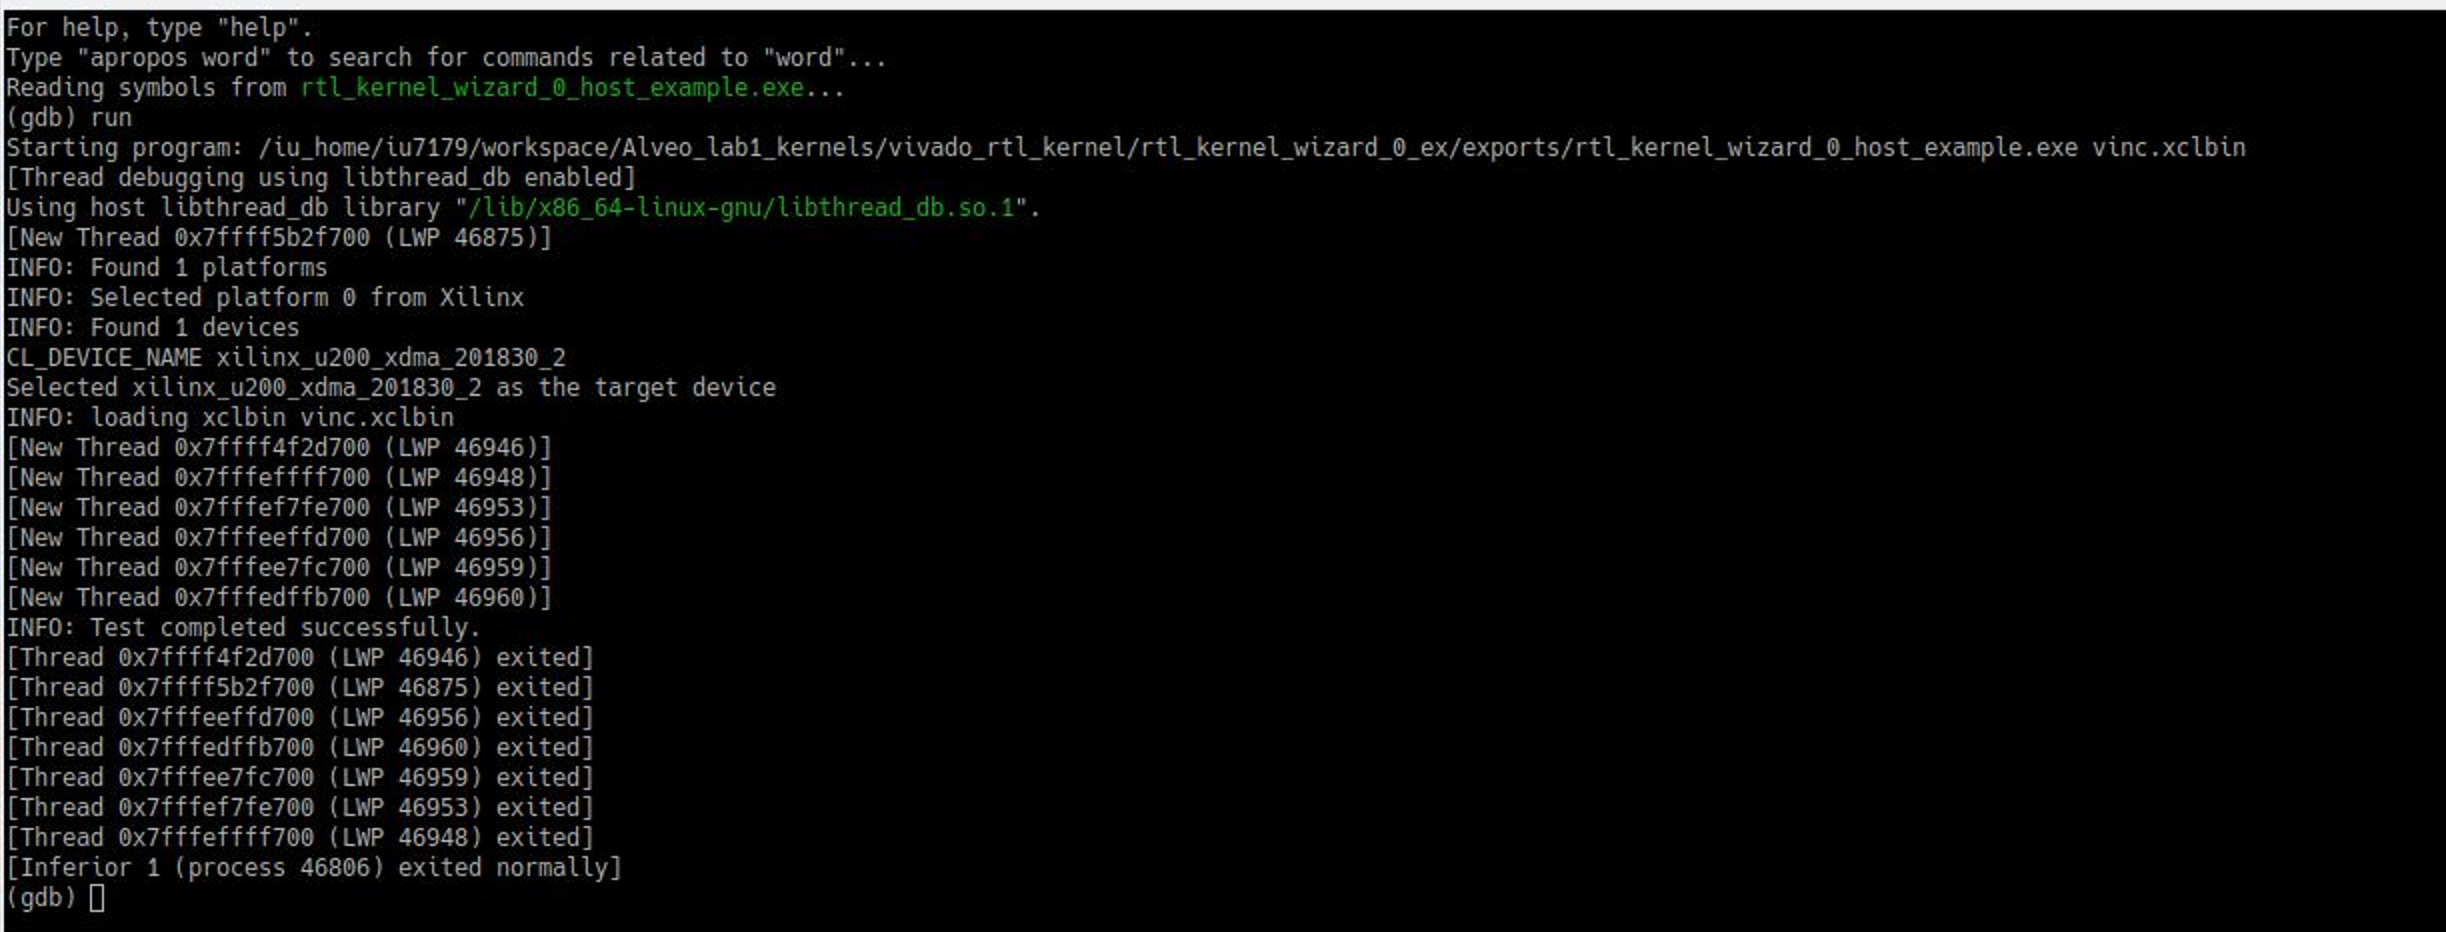
\includegraphics[width = \linewidth]{inc/test.png}
	\caption{Результаты тестирования}
	\label{img:test}
\end{figure}


%\include{30-design}
%\include{40-impl}
%\include{50-research}

\backmatter %% Здесь заканчивается нумерованная часть документа и начинаются ссылки и
            
\StructuredChapter{Заключение}

В ходе данной работы были изучены архитектура гетерогенных вычислительных систем и технологии разработки ускорителей вычислений на базе ПЛИС фирмы Xilinx. Была выполнена генерация ядра ускорителя с последующими синтезом, сборкой и тестированием бинарного модуля ускорителя.
 %% заключение
            
\StructuredChapter{Ответы на контрольные вопросы}

\textbf{1. Преимущества и недостатки XDMA и QDMA платформ}

%Преимущества использовани XDMA:
%\begin{itemize}
%	\item Проще работать
%\end{itemize}

Недостатки использовани XDMA:
\begin{enumerate}
	\item Большая латентность и меньшая пропускная способность за счет того, что данные сначало должны быть перемещены в память ускорителя.
\end{enumerate}

Преимущества использования QDMA:
\begin{enumerate}
	\item Предоставляет прямое потоковое соединение с низкой задержкой и большой пропускной способностью между хостом и ядрами;
	\item Позволяет передавать поток данных непосредственно в логику FPGA параллельно с их обработкой.
\end{enumerate}

%Недостатки использования QDMA:
%\begin{itemize}
%	\item Требуется организовать очередь на хост-устройстве.
%\end{itemize}

\textbf{2. Последовательность действий, необходимых для инициализации ускорителя со стороны хост-системы}

\begin{enumerate}
	\item С помощью вызова clGetPlatformIDs хост получает все платформы.
	\item С помощью вызова clGetPlatformInfo хост получает имя платформы и затем выбирает  платформу Xilinx.
	\item С помощью вызова clGetDeviceIDs хост получает ID устройства.
	\item С помощью вызова clGetDeviceInfo хост получает информацию об устройстве.
	\item С помощью вызова clCreateContext создается контекст для переменных.
	\item С помощью вызова clCreateCommandQueue создается команда для устройтво-ускорителя.
\end{enumerate}

\textbf{3. Процедура запуска задания на исполнения в ускорительном ядре VINC}

\begin{enumerate}
	\item С помощью вызова load\_file\_to\_memory данные, бинарный поток (данные из *.xclbin), копируются из ОЗУ в локальную память ускорителя посредством DMA.
	\item По итогу выполнения clCreateProgramWithBinary, clBuildProgram и clCreateKernel  создается исполняемый файл (уже в памяти устройства-ускорителя).
	\item С помощью clCreateBuffer и clEnqueueWriteBuffer данные, подлежащие обработке, копируются из ОЗУ в локальную память ускорителя посредством DMA (с помощью второй команды осуществляется передача указателей на начало буферов исходных операндов).
	\item С помощью двух вызовов clSetKernelArg указываются параметры (в данном случае это d\_scalar00 и d\_axi00\_ptr0).
	\item С помощью команды clEnqueueNDRangeKernel запускается исполнение ядра (программы на ускорителе).
	\item С помощью команды clEnqueueReadBuffer выполняется чтение готовых данных.
\end{enumerate}

\textbf{4. Процесс линковки на основании содержимого log-файла}

Процесс сборки состоит из шести этапов.
\begin{enumerate}
	\item Анализ конфигурационного файла, анализ профиля устройства, поиск необходимых аппаратных компонентов, интерфейсов;
	\item FPGA линковка синтезированных ядер с платформой;
	\item FPGA оптимизация логики (минимизация логики (булевой) для оптимизации площади, минимизации задержек);
	\item FPGA logic placement (Преобразование булевых уравнений в схему логики ПЛИС. Выбор конкретного места для каждого логического блока в ПЛИС);
	\item FPGA разводка (создание соединений между логическими блоками);
	\item FPGA генерирование файла с программной информацией для отправки его на ПЛИС (*.xclbin файл);
\end{enumerate}
 %% заключение

\appendix   % Тут идут приложения

\chapter{Содержимое файла host\_example.cpp}
\label{cha:appendix1}

\begin{lstlisting}[label=code:hostexample3, caption=Содержимое файла host\_example.cpp, breakatwhitespace=false]
// This is a generated file. Use and modify at your own risk.
////////////////////////////////////////////////////////////////////////////////

/*******************************************************************************
Vendor: Xilinx
Associated Filename: main.c
#Purpose: This example shows a basic vector add +1 (constant) by manipulating
#         memory inplace.
*******************************************************************************/

#include <fcntl.h>
#include <stdio.h>
#include <iostream>
#include <stdlib.h>
#include <string.h>
#include <math.h>
#ifdef _WINDOWS
#include <io.h>
#else
#include <unistd.h>
#include <sys/time.h>
#endif
#include <assert.h>
#include <stdbool.h>
#include <sys/types.h>
#include <sys/stat.h>
#include <CL/opencl.h>
#include <CL/cl_ext.h>
#include "xclhal2.h"

////////////////////////////////////////////////////////////////////////////////

#define NUM_WORKGROUPS (1)
#define WORKGROUP_SIZE (256)
#define MAX_LENGTH 8192
#define MEM_ALIGNMENT 4096
#if defined(VITIS_PLATFORM) && !defined(TARGET_DEVICE)
#define STR_VALUE(arg)      #arg
#define GET_STRING(name) STR_VALUE(name)
#define TARGET_DEVICE GET_STRING(VITIS_PLATFORM)
#endif

////////////////////////////////////////////////////////////////////////////////

cl_uint load_file_to_memory(const char *filename, char **result)
{
    cl_uint size = 0;
    FILE *f = fopen(filename, "rb");
    if (f == NULL) {
        *result = NULL;
        return -1; // -1 means file opening fail
    }
    fseek(f, 0, SEEK_END);
    size = ftell(f);
    fseek(f, 0, SEEK_SET);
    *result = (char *)malloc(size+1);
    if (size != fread(*result, sizeof(char), size, f)) {
        free(*result);
        return -2; // -2 means file reading fail
    }
    fclose(f);
    (*result)[size] = 0;
    return size;
}

int main(int argc, char** argv)
{

    cl_int err;                            // error code returned from api calls
    cl_uint check_status = 0;
    const cl_uint number_of_words = 4096; // 16KB of data


    cl_platform_id platform_id;         // platform id
    cl_device_id device_id;             // compute device id
    cl_context context;                 // compute context
    cl_command_queue commands;          // compute command queue
    cl_program program;                 // compute programs
    cl_kernel kernel;                   // compute kernel

    cl_uint* h_data;                                // host memory for input vector
    char cl_platform_vendor[1001];
    char target_device_name[1001] = TARGET_DEVICE;

    cl_uint* h_axi00_ptr0_output = (cl_uint*)aligned_alloc(MEM_ALIGNMENT,MAX_LENGTH * sizeof(cl_uint*)); // host memory for output vector
    cl_mem d_axi00_ptr0;                         // device memory used for a vector

    if (argc != 2) {
        printf("Usage: %s xclbin\n", argv[0]);
        return EXIT_FAILURE;
    }

    // Fill our data sets with pattern
    h_data = (cl_uint*)aligned_alloc(MEM_ALIGNMENT,MAX_LENGTH * sizeof(cl_uint*));
    for(cl_uint i = 0; i < MAX_LENGTH; i++) {
        h_data[i]  = i;
        h_axi00_ptr0_output[i] = 0; 

    }

    // Get all platforms and then select Xilinx platform
    cl_platform_id platforms[16];       // platform id
    cl_uint platform_count;
    cl_uint platform_found = 0;
    err = clGetPlatformIDs(16, platforms, &platform_count);
    if (err != CL_SUCCESS) {
        printf("ERROR: Failed to find an OpenCL platform!\n");
        printf("ERROR: Test failed\n");
        return EXIT_FAILURE;
    }
    printf("INFO: Found %d platforms\n", platform_count);

    // Find Xilinx Plaftorm
    for (cl_uint iplat=0; iplat<platform_count; iplat++) {
        err = clGetPlatformInfo(platforms[iplat], CL_PLATFORM_VENDOR, 1000, (void *)cl_platform_vendor,NULL);
        if (err != CL_SUCCESS) {
            printf("ERROR: clGetPlatformInfo(CL_PLATFORM_VENDOR) failed!\n");
            printf("ERROR: Test failed\n");
            return EXIT_FAILURE;
        }
        if (strcmp(cl_platform_vendor, "Xilinx") == 0) {
            printf("INFO: Selected platform %d from %s\n", iplat, cl_platform_vendor);
            platform_id = platforms[iplat];
            platform_found = 1;
        }
    }
    if (!platform_found) {
        printf("ERROR: Platform Xilinx not found. Exit.\n");
        return EXIT_FAILURE;
    }

    // Get Accelerator compute device
    cl_uint num_devices;
    cl_uint device_found = 0;
    cl_device_id devices[16];  // compute device id
    char cl_device_name[1001];
    err = clGetDeviceIDs(platform_id, CL_DEVICE_TYPE_ACCELERATOR, 16, devices, &num_devices);
    printf("INFO: Found %d devices\n", num_devices);
    if (err != CL_SUCCESS) {
        printf("ERROR: Failed to create a device group!\n");
        printf("ERROR: Test failed\n");
        return -1;
    }

    //iterate all devices to select the target device.
    for (cl_uint i=0; i<num_devices; i++) {
        err = clGetDeviceInfo(devices[i], CL_DEVICE_NAME, 1024, cl_device_name, 0);
        if (err != CL_SUCCESS) {
            printf("ERROR: Failed to get device name for device %d!\n", i);
            printf("ERROR: Test failed\n");
            return EXIT_FAILURE;
        }
        printf("CL_DEVICE_NAME %s\n", cl_device_name);
        if(strcmp(cl_device_name, target_device_name) == 0) {
            device_id = devices[i];
            device_found = 1;
            printf("Selected %s as the target device\n", cl_device_name);
        }
    }

    if (!device_found) {
        printf("ERROR:Target device %s not found. Exit.\n", target_device_name);
        return EXIT_FAILURE;
    }

    // Create a compute context
    //
    context = clCreateContext(0, 1, &device_id, NULL, NULL, &err);
    if (!context) {
        printf("ERROR: Failed to create a compute context!\n");
        printf("ERROR: Test failed\n");
        return EXIT_FAILURE;
    }

    // Create a command commands
    commands = clCreateCommandQueue(context, device_id, CL_QUEUE_PROFILING_ENABLE | CL_QUEUE_OUT_OF_ORDER_EXEC_MODE_ENABLE, &err);
    if (!commands) {
        printf("ERROR: Failed to create a command commands!\n");
        printf("ERROR: code %i\n",err);
        printf("ERROR: Test failed\n");
        return EXIT_FAILURE;
    }

    cl_int status;

    // Create Program Objects
    // Load binary from disk
    unsigned char *kernelbinary;
    char *xclbin = argv[1];

    //------------------------------------------------------------------------------
    // xclbin
    //------------------------------------------------------------------------------
    printf("INFO: loading xclbin %s\n", xclbin);
    cl_uint n_i0 = load_file_to_memory(xclbin, (char **) &kernelbinary);
    if (n_i0 < 0) {
        printf("ERROR: failed to load kernel from xclbin: %s\n", xclbin);
        printf("ERROR: Test failed\n");
        return EXIT_FAILURE;
    }

    size_t n0 = n_i0;

    // Create the compute program from offline
    program = clCreateProgramWithBinary(context, 1, &device_id, &n0,
                                        (const unsigned char **) &kernelbinary, &status, &err);
    free(kernelbinary);

    if ((!program) || (err!=CL_SUCCESS)) {
        printf("ERROR: Failed to create compute program from binary %d!\n", err);
        printf("ERROR: Test failed\n");
        return EXIT_FAILURE;
    }


    // Build the program executable
    //
    err = clBuildProgram(program, 0, NULL, NULL, NULL, NULL);
    if (err != CL_SUCCESS) {
        size_t len;
        char buffer[2048];

        printf("ERROR: Failed to build program executable!\n");
        clGetProgramBuildInfo(program, device_id, CL_PROGRAM_BUILD_LOG, sizeof(buffer), buffer, &len);
        printf("%s\n", buffer);
        printf("ERROR: Test failed\n");
        return EXIT_FAILURE;
    }

    // Create the compute kernel in the program we wish to run
    //
    kernel = clCreateKernel(program, "rtl_kernel_wizard_0", &err);
    if (!kernel || err != CL_SUCCESS) {
        printf("ERROR: Failed to create compute kernel!\n");
        printf("ERROR: Test failed\n");
        return EXIT_FAILURE;
    }

    // Create structs to define memory bank mapping
    cl_mem_ext_ptr_t mem_ext;
    mem_ext.obj = NULL;
    mem_ext.param = kernel;


    mem_ext.flags = 1;
    d_axi00_ptr0 = clCreateBuffer(context,  CL_MEM_READ_WRITE | CL_MEM_EXT_PTR_XILINX,  sizeof(cl_uint) * number_of_words, &mem_ext, &err);
    if (err != CL_SUCCESS) {
      std::cout << "Return code for clCreateBuffer flags=" << mem_ext.flags << ": " << err << std::endl;
    }


    if (!(d_axi00_ptr0)) {
        printf("ERROR: Failed to allocate device memory!\n");
        printf("ERROR: Test failed\n");
        return EXIT_FAILURE;
    }


    err = clEnqueueWriteBuffer(commands, d_axi00_ptr0, CL_TRUE, 0, sizeof(cl_uint) * number_of_words, h_data, 0, NULL, NULL);
    if (err != CL_SUCCESS) {
        printf("ERROR: Failed to write to source array h_data: d_axi00_ptr0: %d!\n", err);
        printf("ERROR: Test failed\n");
        return EXIT_FAILURE;
    }


    // Set the arguments to our compute kernel
    // cl_uint vector_length = MAX_LENGTH;
    err = 0;
    cl_uint d_scalar00 = 0;
    err |= clSetKernelArg(kernel, 0, sizeof(cl_uint), &d_scalar00); // Not used in example RTL logic.
    err |= clSetKernelArg(kernel, 1, sizeof(cl_mem), &d_axi00_ptr0); 

    if (err != CL_SUCCESS) {
        printf("ERROR: Failed to set kernel arguments! %d\n", err);
        printf("ERROR: Test failed\n");
        return EXIT_FAILURE;
    }

    size_t global[1];
    size_t local[1];
    // Execute the kernel over the entire range of our 1d input data set
    // using the maximum number of work group items for this device

    global[0] = 1;
    local[0] = 1;
    err = clEnqueueNDRangeKernel(commands, kernel, 1, NULL, (size_t*)&global, (size_t*)&local, 0, NULL, NULL);
    if (err) {
        printf("ERROR: Failed to execute kernel! %d\n", err);
        printf("ERROR: Test failed\n");
        return EXIT_FAILURE;
    }

    clFinish(commands);


    // Read back the results from the device to verify the output
    //
    cl_event readevent;

    err = 0;
    err |= clEnqueueReadBuffer( commands, d_axi00_ptr0, CL_TRUE, 0, sizeof(cl_uint) * number_of_words, h_axi00_ptr0_output, 0, NULL, &readevent );


    if (err != CL_SUCCESS) {
        printf("ERROR: Failed to read output array! %d\n", err);
        printf("ERROR: Test failed\n");
        return EXIT_FAILURE;
    }
    clWaitForEvents(1, &readevent);
    // Check Results

    for (cl_uint i = 0; i < number_of_words; i++) {
        unsigned res = (h_data[i] > 61680 ? h_data[i] : 61680) + 1;
        if (res != h_axi00_ptr0_output[i]) {
            printf("ERROR in rtl_kernel_wizard_0::m00_axi - array index %d (host addr 0x%03x) - input=%d (0x%x), output=%d (0x%x)\n", i, i*4, h_data[i], h_data[i], h_axi00_ptr0_output[i], h_axi00_ptr0_output[i]);
            check_status = 1;
        }
      //  printf("i=%d, input=%d, output=%d\n", i,  h_axi00_ptr0_input[i], h_axi00_ptr0_output[i]);
    }


    //--------------------------------------------------------------------------
    // Shutdown and cleanup
    //-------------------------------------------------------------------------- 
    clReleaseMemObject(d_axi00_ptr0);
    free(h_axi00_ptr0_output);



    free(h_data);
    clReleaseProgram(program);
    clReleaseKernel(kernel);
    clReleaseCommandQueue(commands);
    clReleaseContext(context);

    if (check_status) {
        printf("ERROR: Test failed\n");
        return EXIT_FAILURE;
    } else {
        printf("INFO: Test completed successfully.\n");
        return EXIT_SUCCESS;
    }


} // end of main
\end{lstlisting}

\chapter{Содержимое xclbin.info-файла}
\label{cha:appendix1}
\begin{lstlisting}[label=func,breakatwhitespace=false,caption=Содержимое vinc.xclbin.info файла.]
==============================================================================
XRT Build Version: 2.8.743 (2020.2)
       Build Date: 2020-11-16 00:19:11
          Hash ID: 77d5484b5c4daa691a7f78235053fb036829b1e9
==============================================================================
xclbin Information
------------------
   Generated by:           v++ (2020.2) on 2020-11-18-05:13:29
   Version:                2.8.743
   Kernels:                rtl_kernel_wizard_0
   Signature:              
   Content:                Bitstream
   UUID (xclbin):          2ad77cd8-9519-4568-938e-8d376acc3ea2
   Sections:               DEBUG_IP_LAYOUT, BITSTREAM, MEM_TOPOLOGY, IP_LAYOUT, 
                           CONNECTIVITY, CLOCK_FREQ_TOPOLOGY, BUILD_METADATA, 
                           EMBEDDED_METADATA, SYSTEM_METADATA, 
                           GROUP_CONNECTIVITY, GROUP_TOPOLOGY
==============================================================================
Hardware Platform (Shell) Information
-------------------------------------
   Vendor:                 xilinx
   Board:                  u200
   Name:                   xdma
   Version:                201830.2
   Generated Version:      Vivado 2018.3 (SW Build: 2568420)
   Created:                Tue Jun 25 06:55:20 2019
   FPGA Device:            xcu200
   Board Vendor:           xilinx.com
   Board Name:             xilinx.com:au200:1.0
   Board Part:             xilinx.com:au200:part0:1.0
   Platform VBNV:          xilinx_u200_xdma_201830_2
   Static UUID:            c102e7af-b2b8-4381-992b-9a00cc3863eb
   Feature ROM TimeStamp:  1561465320

Clocks
------
   Name:      DATA_CLK
   Index:     0
   Type:      DATA
   Frequency: 300 MHz

   Name:      KERNEL_CLK
   Index:     1
   Type:      KERNEL
   Frequency: 500 MHz

Memory Configuration
--------------------
   Name:         bank0
   Index:        0
   Type:         MEM_DDR4
   Base Address: 0x4000000000
   Address Size: 0x400000000
   Bank Used:    No

   Name:         bank1
   Index:        1
   Type:         MEM_DDR4
   Base Address: 0x5000000000
   Address Size: 0x400000000
   Bank Used:    No

   Name:         bank2
   Index:        2
   Type:         MEM_DDR4
   Base Address: 0x6000000000
   Address Size: 0x400000000
   Bank Used:    No

   Name:         bank3
   Index:        3
   Type:         MEM_DDR4
   Base Address: 0x7000000000
   Address Size: 0x400000000
   Bank Used:    Yes

   Name:         PLRAM[0]
   Index:        4
   Type:         MEM_DRAM
   Base Address: 0x3000000000
   Address Size: 0x20000
   Bank Used:    No

   Name:         PLRAM[1]
   Index:        5
   Type:         MEM_DRAM
   Base Address: 0x3000200000
   Address Size: 0x20000
   Bank Used:    No

   Name:         PLRAM[2]
   Index:        6
   Type:         MEM_DRAM
   Base Address: 0x3000400000
   Address Size: 0x20000
   Bank Used:    No
==============================================================================
Kernel: rtl_kernel_wizard_0

Definition
----------
   Signature: rtl_kernel_wizard_0 (uint scalar00, int* axi00_ptr0)

Ports
-----
   Port:          s_axi_control
   Mode:          slave
   Range (bytes): 0x1000
   Data Width:    32 bits
   Port Type:     addressable

   Port:          m00_axi
   Mode:          master
   Range (bytes): 0xFFFFFFFFFFFFFFFF
   Data Width:    512 bits
   Port Type:     addressable

--------------------------
Instance:        vinc0
   Base Address: 0x1e00000

   Argument:          scalar00
   Register Offset:   0x010
   Port:              s_axi_control
   Memory:            <not applicable>

   Argument:          axi00_ptr0
   Register Offset:   0x018
   Port:              m00_axi
   Memory:            bank3 (MEM_DDR4)
==============================================================================
Generated By
------------
   Command:       v++
   Version:       2020.2 - 2020-11-18-05:13:29 (SW BUILD: 0)
   Command Line:  v++ --config /iu_home/iu7179/workspace/Alveo_lab1_kernels/vivado_rtl_kernel/rtl_kernel_wizard_0_ex/exports/myconf.conf --connectivity.nk rtl_kernel_wizard_0:1:vinc0 --connectivity.slr vinc0:SLR2 --connectivity.sp vinc0.m00_axi:DDR[3] --connectivity.sp vinc0.m00_axi:PLRAM[0] --input_files /iu_home/iu7179/workspace/Alveo_lab1_kernels/vivado_rtl_kernel/rtl_kernel_wizard_0_ex/exports/rtl_kernel_wizard_0.xo --link --optimize 0 --output vinc.xclbin --platform xilinx_u200_xdma_201830_2 --report_level 0 --target hw --vivado.prop run.impl_1.STEPS.OPT_DESIGN.ARGS.DIRECTIVE=Explore --vivado.prop run.impl_1.STEPS.PLACE_DESIGN.ARGS.DIRECTIVE=Explore --vivado.prop run.impl_1.STEPS.PHYS_OPT_DESIGN.IS_ENABLED=true --vivado.prop run.impl_1.STEPS.PHYS_OPT_DESIGN.ARGS.DIRECTIVE=AggressiveExplore --vivado.prop run.impl_1.STEPS.ROUTE_DESIGN.ARGS.DIRECTIVE=Explore 
   Options:       --config /iu_home/iu7179/workspace/Alveo_lab1_kernels/vivado_rtl_kernel/rtl_kernel_wizard_0_ex/exports/myconf.conf
                  --connectivity.nk rtl_kernel_wizard_0:1:vinc0
                  --connectivity.slr vinc0:SLR2
                  --connectivity.sp vinc0.m00_axi:DDR[3]
                  --connectivity.sp vinc0.m00_axi:PLRAM[0]
                  --input_files /iu_home/iu7179/workspace/Alveo_lab1_kernels/vivado_rtl_kernel/rtl_kernel_wizard_0_ex/exports/rtl_kernel_wizard_0.xo
                  --link
                  --optimize 0
                  --output vinc.xclbin
                  --platform xilinx_u200_xdma_201830_2
                  --report_level 0
                  --target hw
                  --vivado.prop run.impl_1.STEPS.OPT_DESIGN.ARGS.DIRECTIVE=Explore
                  --vivado.prop run.impl_1.STEPS.PLACE_DESIGN.ARGS.DIRECTIVE=Explore
                  --vivado.prop run.impl_1.STEPS.PHYS_OPT_DESIGN.IS_ENABLED=true
                  --vivado.prop run.impl_1.STEPS.PHYS_OPT_DESIGN.ARGS.DIRECTIVE=AggressiveExplore
                  --vivado.prop run.impl_1.STEPS.ROUTE_DESIGN.ARGS.DIRECTIVE=Explore 
==============================================================================
User Added Key Value Pairs
--------------------------
   <empty>
==============================================================================
\end{lstlisting}
\chapter{Содержимое log-файла}
\label{cha:appendix1}
\begin{lstlisting}[label=func,breaklines=true,breakatwhitespace=false,caption=СОДЕРЖИМОЕ LOG-ФАЙЛА.]
INFO: [v++ 60-1306] Additional information associated with this v++ link can be found at:
	Reports: /iu_home/iu7179/workspace/Alveo_lab1_kernels/vivado_rtl_kernel/rtl_kernel_wizard_0_ex/exports/_x/reports/link
	Log files: /iu_home/iu7179/workspace/Alveo_lab1_kernels/vivado_rtl_kernel/rtl_kernel_wizard_0_ex/exports/_x/logs/link
INFO: [v++ 60-1548] Creating build summary session with primary output /iu_home/iu7179/workspace/Alveo_lab1_kernels/vivado_rtl_kernel/rtl_kernel_wizard_0_ex/exports/vinc.xclbin.link_summary, at Sat Dec 11 11:52:07 2021
INFO: [v++ 60-1316] Initiating connection to rulecheck server, at Sat Dec 11 11:52:07 2021
INFO: [v++ 60-1315] Creating rulecheck session with output '/iu_home/iu7179/workspace/Alveo_lab1_kernels/vivado_rtl_kernel/rtl_kernel_wizard_0_ex/exports/_x/reports/link/v++_link_vinc_guidance.html', at Sat Dec 11 11:52:26 2021
INFO: [v++ 60-895]   Target platform: /opt/xilinx/platforms/xilinx_u200_xdma_201830_2/xilinx_u200_xdma_201830_2.xpfm
INFO: [v++ 60-1578]   This platform contains Device Support Archive '/opt/xilinx/platforms/xilinx_u200_xdma_201830_2/hw/xilinx_u200_xdma_201830_2.dsa'
INFO: [v++ 74-74] Compiler Version string: 2020.2
INFO: [v++ 60-1302] Platform 'xilinx_u200_xdma_201830_2.xpfm' has been explicitly enabled for this release.
INFO: [v++ 60-629] Linking for hardware target
INFO: [v++ 60-423]   Target device: xilinx_u200_xdma_201830_2
INFO: [v++ 60-1332] Run 'run_link' status: Not started
INFO: [v++ 60-1443] [11:53:22] Run run_link: Step system_link: Started
INFO: [v++ 60-1453] Command Line: system_link --xo /iu_home/iu7179/workspace/Alveo_lab1_kernels/vivado_rtl_kernel/rtl_kernel_wizard_0_ex/exports/rtl_kernel_wizard_0.xo --config /iu_home/iu7179/workspace/Alveo_lab1_kernels/vivado_rtl_kernel/rtl_kernel_wizard_0_ex/exports/_x/link/int/syslinkConfig.ini --xpfm /opt/xilinx/platforms/xilinx_u200_xdma_201830_2/xilinx_u200_xdma_201830_2.xpfm --target hw --output_dir /iu_home/iu7179/workspace/Alveo_lab1_kernels/vivado_rtl_kernel/rtl_kernel_wizard_0_ex/exports/_x/link/int --temp_dir /iu_home/iu7179/workspace/Alveo_lab1_kernels/vivado_rtl_kernel/rtl_kernel_wizard_0_ex/exports/_x/link/sys_link
INFO: [v++ 60-1454] Run Directory: /iu_home/iu7179/workspace/Alveo_lab1_kernels/vivado_rtl_kernel/rtl_kernel_wizard_0_ex/exports/_x/link/run_link
INFO: [SYSTEM_LINK 60-1316] Initiating connection to rulecheck server, at Sat Dec 11 11:53:37 2021
INFO: [SYSTEM_LINK 82-70] Extracting xo v3 file /iu_home/iu7179/workspace/Alveo_lab1_kernels/vivado_rtl_kernel/rtl_kernel_wizard_0_ex/exports/rtl_kernel_wizard_0.xo
INFO: [SYSTEM_LINK 82-53] Creating IP database /iu_home/iu7179/workspace/Alveo_lab1_kernels/vivado_rtl_kernel/rtl_kernel_wizard_0_ex/exports/_x/link/sys_link/_sysl/.cdb/xd_ip_db.xml
INFO: [SYSTEM_LINK 82-38] [11:53:39] build_xd_ip_db started: /data/Xilinx/Vitis/2020.2/bin/build_xd_ip_db -ip_search 0  -sds-pf /iu_home/iu7179/workspace/Alveo_lab1_kernels/vivado_rtl_kernel/rtl_kernel_wizard_0_ex/exports/_x/link/sys_link/xilinx_u200_xdma_201830_2.hpfm -clkid 0 -ip /iu_home/iu7179/workspace/Alveo_lab1_kernels/vivado_rtl_kernel/rtl_kernel_wizard_0_ex/exports/_x/link/sys_link/iprepo/mycompany_com_kernel_rtl_kernel_wizard_0_1_0,rtl_kernel_wizard_0 -o /iu_home/iu7179/workspace/Alveo_lab1_kernels/vivado_rtl_kernel/rtl_kernel_wizard_0_ex/exports/_x/link/sys_link/_sysl/.cdb/xd_ip_db.xml
INFO: [SYSTEM_LINK 82-37] [11:54:08] build_xd_ip_db finished successfully
Time (s): cpu = 00:00:30 ; elapsed = 00:00:29 . Memory (MB): peak = 1557.895 ; gain = 0.000 ; free physical = 51564 ; free virtual = 232990
INFO: [SYSTEM_LINK 82-51] Create system connectivity graph
INFO: [SYSTEM_LINK 82-102] Applying explicit connections to the system connectivity graph: /iu_home/iu7179/workspace/Alveo_lab1_kernels/vivado_rtl_kernel/rtl_kernel_wizard_0_ex/exports/_x/link/sys_link/cfgraph/cfgen_cfgraph.xml
INFO: [SYSTEM_LINK 82-38] [11:54:08] cfgen started: /data/Xilinx/Vitis/2020.2/bin/cfgen  -nk rtl_kernel_wizard_0:1:vinc0 -slr vinc0:SLR2 -sp vinc0.m00_axi:DDR[3] -sp vinc0.m00_axi:PLRAM[0] -dmclkid 0 -r /iu_home/iu7179/workspace/Alveo_lab1_kernels/vivado_rtl_kernel/rtl_kernel_wizard_0_ex/exports/_x/link/sys_link/_sysl/.cdb/xd_ip_db.xml -o /iu_home/iu7179/workspace/Alveo_lab1_kernels/vivado_rtl_kernel/rtl_kernel_wizard_0_ex/exports/_x/link/sys_link/cfgraph/cfgen_cfgraph.xml
INFO: [CFGEN 83-0] Kernel Specs: 
INFO: [CFGEN 83-0]   kernel: rtl_kernel_wizard_0, num: 1  {vinc0}
INFO: [CFGEN 83-0] Port Specs: 
INFO: [CFGEN 83-0]   kernel: vinc0, k_port: m00_axi, sptag: DDR[3]
INFO: [CFGEN 83-0]   kernel: vinc0, k_port: m00_axi, sptag: PLRAM[0]
INFO: [CFGEN 83-0] SLR Specs: 
INFO: [CFGEN 83-0]   instance: vinc0, SLR: SLR2
INFO: [CFGEN 83-2228] Creating mapping for argument vinc0.axi00_ptr0 to DDR[3] for directive vinc0.m00_axi:DDR[3]
INFO: [SYSTEM_LINK 82-37] [11:54:30] cfgen finished successfully
Time (s): cpu = 00:00:21 ; elapsed = 00:00:22 . Memory (MB): peak = 1557.895 ; gain = 0.000 ; free physical = 47722 ; free virtual = 229156
INFO: [SYSTEM_LINK 82-52] Create top-level block diagram
INFO: [SYSTEM_LINK 82-38] [11:54:30] cf2bd started: /data/Xilinx/Vitis/2020.2/bin/cf2bd  --linux --trace_buffer 1024 --input_file /iu_home/iu7179/workspace/Alveo_lab1_kernels/vivado_rtl_kernel/rtl_kernel_wizard_0_ex/exports/_x/link/sys_link/cfgraph/cfgen_cfgraph.xml --ip_db /iu_home/iu7179/workspace/Alveo_lab1_kernels/vivado_rtl_kernel/rtl_kernel_wizard_0_ex/exports/_x/link/sys_link/_sysl/.cdb/xd_ip_db.xml --cf_name dr --working_dir /iu_home/iu7179/workspace/Alveo_lab1_kernels/vivado_rtl_kernel/rtl_kernel_wizard_0_ex/exports/_x/link/sys_link/_sysl/.xsd --temp_dir /iu_home/iu7179/workspace/Alveo_lab1_kernels/vivado_rtl_kernel/rtl_kernel_wizard_0_ex/exports/_x/link/sys_link --output_dir /iu_home/iu7179/workspace/Alveo_lab1_kernels/vivado_rtl_kernel/rtl_kernel_wizard_0_ex/exports/_x/link/int --target_bd pfm_dynamic.bd
INFO: [CF2BD 82-31] Launching cf2xd: cf2xd -linux -trace-buffer 1024 -i /iu_home/iu7179/workspace/Alveo_lab1_kernels/vivado_rtl_kernel/rtl_kernel_wizard_0_ex/exports/_x/link/sys_link/cfgraph/cfgen_cfgraph.xml -r /iu_home/iu7179/workspace/Alveo_lab1_kernels/vivado_rtl_kernel/rtl_kernel_wizard_0_ex/exports/_x/link/sys_link/_sysl/.cdb/xd_ip_db.xml -o dr.xml
INFO: [CF2BD 82-28] cf2xd finished successfully
INFO: [CF2BD 82-31] Launching cf_xsd: cf_xsd -disable-address-gen -bd pfm_dynamic.bd -dn dr -dp /iu_home/iu7179/workspace/Alveo_lab1_kernels/vivado_rtl_kernel/rtl_kernel_wizard_0_ex/exports/_x/link/sys_link/_sysl/.xsd
INFO: [CF2BD 82-28] cf_xsd finished successfully
INFO: [SYSTEM_LINK 82-37] [11:54:43] cf2bd finished successfully
Time (s): cpu = 00:00:11 ; elapsed = 00:00:13 . Memory (MB): peak = 1557.895 ; gain = 0.000 ; free physical = 47497 ; free virtual = 228947
INFO: [v++ 60-1441] [11:54:44] Run run_link: Step system_link: Completed
Time (s): cpu = 00:01:18 ; elapsed = 00:01:22 . Memory (MB): peak = 1576.969 ; gain = 0.000 ; free physical = 47563 ; free virtual = 229009
INFO: [v++ 60-1443] [11:54:44] Run run_link: Step cf2sw: Started
INFO: [v++ 60-1453] Command Line: cf2sw -sdsl /iu_home/iu7179/workspace/Alveo_lab1_kernels/vivado_rtl_kernel/rtl_kernel_wizard_0_ex/exports/_x/link/int/sdsl.dat -rtd /iu_home/iu7179/workspace/Alveo_lab1_kernels/vivado_rtl_kernel/rtl_kernel_wizard_0_ex/exports/_x/link/int/cf2sw.rtd -nofilter /iu_home/iu7179/workspace/Alveo_lab1_kernels/vivado_rtl_kernel/rtl_kernel_wizard_0_ex/exports/_x/link/int/cf2sw_full.rtd -xclbin /iu_home/iu7179/workspace/Alveo_lab1_kernels/vivado_rtl_kernel/rtl_kernel_wizard_0_ex/exports/_x/link/int/xclbin_orig.xml -o /iu_home/iu7179/workspace/Alveo_lab1_kernels/vivado_rtl_kernel/rtl_kernel_wizard_0_ex/exports/_x/link/int/xclbin_orig.1.xml
INFO: [v++ 60-1454] Run Directory: /iu_home/iu7179/workspace/Alveo_lab1_kernels/vivado_rtl_kernel/rtl_kernel_wizard_0_ex/exports/_x/link/run_link
INFO: [v++ 60-1441] [11:54:57] Run run_link: Step cf2sw: Completed
Time (s): cpu = 00:00:13 ; elapsed = 00:00:14 . Memory (MB): peak = 1576.969 ; gain = 0.000 ; free physical = 46909 ; free virtual = 228364
INFO: [v++ 60-1443] [11:54:57] Run run_link: Step rtd2_system_diagram: Started
INFO: [v++ 60-1453] Command Line: rtd2SystemDiagram
INFO: [v++ 60-1454] Run Directory: /iu_home/iu7179/workspace/Alveo_lab1_kernels/vivado_rtl_kernel/rtl_kernel_wizard_0_ex/exports/_x/link/run_link
INFO: [v++ 60-1441] [11:55:06] Run run_link: Step rtd2_system_diagram: Completed
Time (s): cpu = 00:00:00.01 ; elapsed = 00:00:09 . Memory (MB): peak = 1576.969 ; gain = 0.000 ; free physical = 44422 ; free virtual = 225881
INFO: [v++ 60-1443] [11:55:06] Run run_link: Step vpl: Started
INFO: [v++ 60-1453] Command Line: vpl -t hw -f xilinx_u200_xdma_201830_2 --remote_ip_cache /iu_home/iu7179/workspace/Alveo_lab1_kernels/vivado_rtl_kernel/rtl_kernel_wizard_0_ex/exports/.ipcache --output_dir /iu_home/iu7179/workspace/Alveo_lab1_kernels/vivado_rtl_kernel/rtl_kernel_wizard_0_ex/exports/_x/link/int --log_dir /iu_home/iu7179/workspace/Alveo_lab1_kernels/vivado_rtl_kernel/rtl_kernel_wizard_0_ex/exports/_x/logs/link --report_dir /iu_home/iu7179/workspace/Alveo_lab1_kernels/vivado_rtl_kernel/rtl_kernel_wizard_0_ex/exports/_x/reports/link --config /iu_home/iu7179/workspace/Alveo_lab1_kernels/vivado_rtl_kernel/rtl_kernel_wizard_0_ex/exports/_x/link/int/vplConfig.ini -k /iu_home/iu7179/workspace/Alveo_lab1_kernels/vivado_rtl_kernel/rtl_kernel_wizard_0_ex/exports/_x/link/int/kernel_info.dat --webtalk_flag Vitis --temp_dir /iu_home/iu7179/workspace/Alveo_lab1_kernels/vivado_rtl_kernel/rtl_kernel_wizard_0_ex/exports/_x/link --no-info --iprepo /iu_home/iu7179/workspace/Alveo_lab1_kernels/vivado_rtl_kernel/rtl_kernel_wizard_0_ex/exports/_x/link/int/xo/ip_repo/mycompany_com_kernel_rtl_kernel_wizard_0_1_0 --messageDb /iu_home/iu7179/workspace/Alveo_lab1_kernels/vivado_rtl_kernel/rtl_kernel_wizard_0_ex/exports/_x/link/run_link/vpl.pb /iu_home/iu7179/workspace/Alveo_lab1_kernels/vivado_rtl_kernel/rtl_kernel_wizard_0_ex/exports/_x/link/int/dr.bd.tcl
INFO: [v++ 60-1454] Run Directory: /iu_home/iu7179/workspace/Alveo_lab1_kernels/vivado_rtl_kernel/rtl_kernel_wizard_0_ex/exports/_x/link/run_link

****** vpl v2020.2 (64-bit)
  **** SW Build (by xbuild) on 2020-11-18-05:13:29
    ** Copyright 1986-2020 Xilinx, Inc. All Rights Reserved.

INFO: [VPL 60-839] Read in kernel information from file '/iu_home/iu7179/workspace/Alveo_lab1_kernels/vivado_rtl_kernel/rtl_kernel_wizard_0_ex/exports/_x/link/int/kernel_info.dat'.
INFO: [VPL 74-74] Compiler Version string: 2020.2
INFO: [VPL 60-423]   Target device: xilinx_u200_xdma_201830_2
INFO: [VPL 60-1032] Extracting hardware platform to /iu_home/iu7179/workspace/Alveo_lab1_kernels/vivado_rtl_kernel/rtl_kernel_wizard_0_ex/exports/_x/link/vivado/vpl/.local/hw_platform
WARNING: /data/Xilinx/Vitis/2020.2/tps/lnx64/jre9.0.4 does not exist.
[11:59:47] Run vpl: Step create_project: Started
Creating Vivado project.
[12:00:13] Run vpl: Step create_project: Completed
[12:00:13] Run vpl: Step create_bd: Started
[12:01:46] Run vpl: Step create_bd: RUNNING...
[12:03:19] Run vpl: Step create_bd: RUNNING...
[12:04:51] Run vpl: Step create_bd: RUNNING...
[12:06:41] Run vpl: Step create_bd: RUNNING...
[12:08:21] Run vpl: Step create_bd: RUNNING...
[12:09:26] Run vpl: Step create_bd: Completed
[12:09:26] Run vpl: Step update_bd: Started
[12:09:30] Run vpl: Step update_bd: Completed
[12:09:30] Run vpl: Step generate_target: Started
[12:11:07] Run vpl: Step generate_target: RUNNING...
[12:12:41] Run vpl: Step generate_target: RUNNING...
[12:14:11] Run vpl: Step generate_target: RUNNING...
[12:15:46] Run vpl: Step generate_target: RUNNING...
[12:17:15] Run vpl: Step generate_target: RUNNING...
[12:18:53] Run vpl: Step generate_target: RUNNING...
[12:20:22] Run vpl: Step generate_target: RUNNING...
[12:22:07] Run vpl: Step generate_target: RUNNING...
[12:22:09] Run vpl: Step generate_target: Completed
[12:22:09] Run vpl: Step config_hw_runs: Started
[12:23:50] Run vpl: Step config_hw_runs: RUNNING...
[12:24:06] Run vpl: Step config_hw_runs: Completed
[12:24:06] Run vpl: Step synth: Started
[12:26:25] Block-level synthesis in progress, 0 of 66 jobs complete, 3 jobs running.
[12:27:02] Block-level synthesis in progress, 0 of 66 jobs complete, 8 jobs running.
[12:27:40] Block-level synthesis in progress, 0 of 66 jobs complete, 8 jobs running.
[12:28:17] Block-level synthesis in progress, 0 of 66 jobs complete, 8 jobs running.
[12:29:00] Block-level synthesis in progress, 0 of 66 jobs complete, 8 jobs running.
[12:29:39] Block-level synthesis in progress, 0 of 66 jobs complete, 8 jobs running.
[12:30:18] Block-level synthesis in progress, 0 of 66 jobs complete, 8 jobs running.
[12:30:55] Block-level synthesis in progress, 0 of 66 jobs complete, 8 jobs running.
[12:31:36] Block-level synthesis in progress, 0 of 66 jobs complete, 8 jobs running.
[12:32:14] Block-level synthesis in progress, 0 of 66 jobs complete, 8 jobs running.
[12:32:53] Block-level synthesis in progress, 0 of 66 jobs complete, 8 jobs running.
[12:33:30] Block-level synthesis in progress, 0 of 66 jobs complete, 8 jobs running.
[12:34:11] Block-level synthesis in progress, 0 of 66 jobs complete, 8 jobs running.
[12:34:48] Block-level synthesis in progress, 0 of 66 jobs complete, 8 jobs running.
[12:35:29] Block-level synthesis in progress, 6 of 66 jobs complete, 2 jobs running.
[12:36:07] Block-level synthesis in progress, 7 of 66 jobs complete, 1 job running.
[12:36:48] Block-level synthesis in progress, 7 of 66 jobs complete, 4 jobs running.
[12:37:27] Block-level synthesis in progress, 7 of 66 jobs complete, 8 jobs running.
[12:38:06] Block-level synthesis in progress, 9 of 66 jobs complete, 6 jobs running.
[12:38:43] Block-level synthesis in progress, 10 of 66 jobs complete, 5 jobs running.
[12:39:24] Block-level synthesis in progress, 10 of 66 jobs complete, 7 jobs running.
[12:40:00] Block-level synthesis in progress, 11 of 66 jobs complete, 7 jobs running.
[12:40:38] Block-level synthesis in progress, 12 of 66 jobs complete, 6 jobs running.
[12:41:17] Block-level synthesis in progress, 12 of 66 jobs complete, 6 jobs running.
[12:41:58] Block-level synthesis in progress, 12 of 66 jobs complete, 8 jobs running.
[12:42:35] Block-level synthesis in progress, 13 of 66 jobs complete, 7 jobs running.
[12:43:18] Block-level synthesis in progress, 13 of 66 jobs complete, 7 jobs running.
[12:43:57] Block-level synthesis in progress, 13 of 66 jobs complete, 7 jobs running.
[12:44:34] Block-level synthesis in progress, 13 of 66 jobs complete, 8 jobs running.
[12:45:13] Block-level synthesis in progress, 16 of 66 jobs complete, 5 jobs running.
[12:45:52] Block-level synthesis in progress, 17 of 66 jobs complete, 4 jobs running.
[12:46:31] Block-level synthesis in progress, 18 of 66 jobs complete, 6 jobs running.
[12:47:07] Block-level synthesis in progress, 18 of 66 jobs complete, 7 jobs running.
[12:47:45] Block-level synthesis in progress, 19 of 66 jobs complete, 7 jobs running.
[12:48:21] Block-level synthesis in progress, 19 of 66 jobs complete, 7 jobs running.
[12:48:59] Block-level synthesis in progress, 21 of 66 jobs complete, 6 jobs running.
[12:49:37] Block-level synthesis in progress, 21 of 66 jobs complete, 6 jobs running.
[12:50:16] Block-level synthesis in progress, 21 of 66 jobs complete, 8 jobs running.
[12:50:53] Block-level synthesis in progress, 22 of 66 jobs complete, 7 jobs running.
[12:51:34] Block-level synthesis in progress, 22 of 66 jobs complete, 7 jobs running.
[12:52:10] Block-level synthesis in progress, 22 of 66 jobs complete, 8 jobs running.
[12:52:48] Block-level synthesis in progress, 22 of 66 jobs complete, 8 jobs running.
[12:53:23] Block-level synthesis in progress, 22 of 66 jobs complete, 8 jobs running.
[12:54:03] Block-level synthesis in progress, 24 of 66 jobs complete, 6 jobs running.
[12:54:39] Block-level synthesis in progress, 25 of 66 jobs complete, 5 jobs running.
[12:55:19] Block-level synthesis in progress, 25 of 66 jobs complete, 7 jobs running.
[12:55:55] Block-level synthesis in progress, 25 of 66 jobs complete, 8 jobs running.
[12:56:35] Block-level synthesis in progress, 27 of 66 jobs complete, 6 jobs running.
[12:57:12] Block-level synthesis in progress, 27 of 66 jobs complete, 6 jobs running.
[12:57:51] Block-level synthesis in progress, 29 of 66 jobs complete, 6 jobs running.
[12:58:26] Block-level synthesis in progress, 29 of 66 jobs complete, 6 jobs running.
[12:59:15] Block-level synthesis in progress, 29 of 66 jobs complete, 8 jobs running.
[12:59:52] Block-level synthesis in progress, 30 of 66 jobs complete, 7 jobs running.
[13:00:54] Block-level synthesis in progress, 31 of 66 jobs complete, 6 jobs running.
[13:01:39] Block-level synthesis in progress, 31 of 66 jobs complete, 8 jobs running.
[13:02:15] Block-level synthesis in progress, 32 of 66 jobs complete, 7 jobs running.
[13:02:55] Block-level synthesis in progress, 32 of 66 jobs complete, 7 jobs running.
[13:03:33] Block-level synthesis in progress, 33 of 66 jobs complete, 7 jobs running.
[13:04:13] Block-level synthesis in progress, 33 of 66 jobs complete, 7 jobs running.
[13:04:50] Block-level synthesis in progress, 33 of 66 jobs complete, 8 jobs running.
[13:05:31] Block-level synthesis in progress, 33 of 66 jobs complete, 8 jobs running.
[13:06:10] Block-level synthesis in progress, 34 of 66 jobs complete, 7 jobs running.
[13:06:52] Block-level synthesis in progress, 36 of 66 jobs complete, 5 jobs running.
[13:07:31] Block-level synthesis in progress, 36 of 66 jobs complete, 6 jobs running.
[13:08:13] Block-level synthesis in progress, 36 of 66 jobs complete, 8 jobs running.
[13:08:48] Block-level synthesis in progress, 36 of 66 jobs complete, 8 jobs running.
[13:09:27] Block-level synthesis in progress, 37 of 66 jobs complete, 7 jobs running.
[13:10:06] Block-level synthesis in progress, 38 of 66 jobs complete, 6 jobs running.
[13:10:50] Block-level synthesis in progress, 39 of 66 jobs complete, 6 jobs running.
[13:11:26] Block-level synthesis in progress, 39 of 66 jobs complete, 7 jobs running.
[13:12:06] Block-level synthesis in progress, 39 of 66 jobs complete, 8 jobs running.
[13:12:44] Block-level synthesis in progress, 40 of 66 jobs complete, 7 jobs running.
[13:13:24] Block-level synthesis in progress, 40 of 66 jobs complete, 7 jobs running.
[13:14:00] Block-level synthesis in progress, 40 of 66 jobs complete, 8 jobs running.
[13:14:42] Block-level synthesis in progress, 40 of 66 jobs complete, 8 jobs running.
[13:15:19] Block-level synthesis in progress, 40 of 66 jobs complete, 8 jobs running.
[13:16:01] Block-level synthesis in progress, 41 of 66 jobs complete, 7 jobs running.
[13:16:40] Block-level synthesis in progress, 41 of 66 jobs complete, 7 jobs running.
[13:17:20] Block-level synthesis in progress, 41 of 66 jobs complete, 8 jobs running.
[13:17:55] Block-level synthesis in progress, 42 of 66 jobs complete, 7 jobs running.
[13:18:36] Block-level synthesis in progress, 42 of 66 jobs complete, 7 jobs running.
[13:19:15] Block-level synthesis in progress, 43 of 66 jobs complete, 7 jobs running.
[13:19:54] Block-level synthesis in progress, 43 of 66 jobs complete, 7 jobs running.
[13:20:30] Block-level synthesis in progress, 44 of 66 jobs complete, 7 jobs running.
[13:21:12] Block-level synthesis in progress, 45 of 66 jobs complete, 6 jobs running.
[13:21:49] Block-level synthesis in progress, 46 of 66 jobs complete, 7 jobs running.
[13:22:28] Block-level synthesis in progress, 46 of 66 jobs complete, 7 jobs running.
[13:23:05] Block-level synthesis in progress, 46 of 66 jobs complete, 8 jobs running.
[13:23:45] Block-level synthesis in progress, 46 of 66 jobs complete, 8 jobs running.
[13:24:22] Block-level synthesis in progress, 46 of 66 jobs complete, 8 jobs running.
[13:25:03] Block-level synthesis in progress, 48 of 66 jobs complete, 6 jobs running.
[13:25:40] Block-level synthesis in progress, 48 of 66 jobs complete, 6 jobs running.
[13:26:19] Block-level synthesis in progress, 49 of 66 jobs complete, 7 jobs running.
[13:26:55] Block-level synthesis in progress, 50 of 66 jobs complete, 6 jobs running.
[13:27:34] Block-level synthesis in progress, 51 of 66 jobs complete, 7 jobs running.
[13:28:10] Block-level synthesis in progress, 51 of 66 jobs complete, 7 jobs running.
[13:28:51] Block-level synthesis in progress, 53 of 66 jobs complete, 6 jobs running.
[13:29:27] Block-level synthesis in progress, 55 of 66 jobs complete, 5 jobs running.
[13:30:08] Block-level synthesis in progress, 57 of 66 jobs complete, 6 jobs running.
[13:30:47] Block-level synthesis in progress, 58 of 66 jobs complete, 5 jobs running.
[13:31:28] Block-level synthesis in progress, 59 of 66 jobs complete, 6 jobs running.
[13:32:05] Block-level synthesis in progress, 59 of 66 jobs complete, 6 jobs running.
[13:32:53] Block-level synthesis in progress, 59 of 66 jobs complete, 6 jobs running.
[13:33:29] Block-level synthesis in progress, 60 of 66 jobs complete, 5 jobs running.
[13:34:11] Block-level synthesis in progress, 60 of 66 jobs complete, 5 jobs running.
[13:34:48] Block-level synthesis in progress, 61 of 66 jobs complete, 4 jobs running.
[13:35:29] Block-level synthesis in progress, 61 of 66 jobs complete, 4 jobs running.
[13:36:05] Block-level synthesis in progress, 61 of 66 jobs complete, 4 jobs running.
[13:36:50] Block-level synthesis in progress, 61 of 66 jobs complete, 4 jobs running.
[13:37:30] Block-level synthesis in progress, 62 of 66 jobs complete, 3 jobs running.
[13:38:15] Block-level synthesis in progress, 63 of 66 jobs complete, 2 jobs running.
[13:38:54] Block-level synthesis in progress, 63 of 66 jobs complete, 2 jobs running.
[13:39:40] Block-level synthesis in progress, 63 of 66 jobs complete, 2 jobs running.
[13:40:17] Block-level synthesis in progress, 63 of 66 jobs complete, 2 jobs running.
[13:41:01] Block-level synthesis in progress, 64 of 66 jobs complete, 1 job running.
[13:41:38] Block-level synthesis in progress, 64 of 66 jobs complete, 1 job running.
[13:42:24] Block-level synthesis in progress, 64 of 66 jobs complete, 1 job running.
[13:43:02] Block-level synthesis in progress, 64 of 66 jobs complete, 1 job running.
[13:43:46] Block-level synthesis in progress, 64 of 66 jobs complete, 1 job running.
[13:44:24] Block-level synthesis in progress, 64 of 66 jobs complete, 1 job running.
[13:45:07] Block-level synthesis in progress, 64 of 66 jobs complete, 1 job running.
[13:45:44] Block-level synthesis in progress, 64 of 66 jobs complete, 1 job running.
[13:46:28] Block-level synthesis in progress, 64 of 66 jobs complete, 1 job running.
[13:47:05] Block-level synthesis in progress, 64 of 66 jobs complete, 1 job running.
[13:47:48] Block-level synthesis in progress, 64 of 66 jobs complete, 1 job running.
[13:48:24] Block-level synthesis in progress, 64 of 66 jobs complete, 1 job running.
[13:49:05] Block-level synthesis in progress, 64 of 66 jobs complete, 1 job running.
[13:49:44] Block-level synthesis in progress, 64 of 66 jobs complete, 1 job running.
[13:50:27] Block-level synthesis in progress, 64 of 66 jobs complete, 1 job running.
[13:51:05] Block-level synthesis in progress, 64 of 66 jobs complete, 1 job running.
[13:51:50] Block-level synthesis in progress, 64 of 66 jobs complete, 1 job running.
[13:52:27] Block-level synthesis in progress, 64 of 66 jobs complete, 1 job running.
[13:53:12] Block-level synthesis in progress, 64 of 66 jobs complete, 1 job running.
[13:53:48] Block-level synthesis in progress, 64 of 66 jobs complete, 1 job running.
[13:54:33] Block-level synthesis in progress, 64 of 66 jobs complete, 1 job running.
[13:55:09] Block-level synthesis in progress, 64 of 66 jobs complete, 1 job running.
[13:55:58] Block-level synthesis in progress, 64 of 66 jobs complete, 1 job running.
[13:56:38] Block-level synthesis in progress, 64 of 66 jobs complete, 1 job running.
[13:57:23] Block-level synthesis in progress, 64 of 66 jobs complete, 1 job running.
[13:58:01] Block-level synthesis in progress, 64 of 66 jobs complete, 1 job running.
[13:58:50] Block-level synthesis in progress, 64 of 66 jobs complete, 1 job running.
[13:59:28] Block-level synthesis in progress, 64 of 66 jobs complete, 1 job running.
[14:00:15] Block-level synthesis in progress, 64 of 66 jobs complete, 1 job running.
[14:00:55] Block-level synthesis in progress, 64 of 66 jobs complete, 1 job running.
[14:01:43] Block-level synthesis in progress, 64 of 66 jobs complete, 1 job running.
[14:02:23] Block-level synthesis in progress, 64 of 66 jobs complete, 1 job running.
[14:03:11] Block-level synthesis in progress, 64 of 66 jobs complete, 1 job running.
[14:03:50] Block-level synthesis in progress, 64 of 66 jobs complete, 1 job running.
[14:04:36] Block-level synthesis in progress, 64 of 66 jobs complete, 1 job running.
[14:05:14] Block-level synthesis in progress, 64 of 66 jobs complete, 1 job running.
[14:06:05] Block-level synthesis in progress, 64 of 66 jobs complete, 1 job running.
[14:06:43] Block-level synthesis in progress, 64 of 66 jobs complete, 1 job running.
[14:07:29] Block-level synthesis in progress, 64 of 66 jobs complete, 1 job running.
[14:08:07] Block-level synthesis in progress, 64 of 66 jobs complete, 1 job running.
[14:08:53] Block-level synthesis in progress, 64 of 66 jobs complete, 1 job running.
[14:09:34] Block-level synthesis in progress, 64 of 66 jobs complete, 1 job running.
[14:10:21] Block-level synthesis in progress, 65 of 66 jobs complete, 0 jobs running.
[14:10:59] Block-level synthesis in progress, 65 of 66 jobs complete, 0 jobs running.
[14:11:46] Block-level synthesis in progress, 65 of 66 jobs complete, 0 jobs running.
[14:12:23] Block-level synthesis in progress, 65 of 66 jobs complete, 1 job running.
[14:13:09] Block-level synthesis in progress, 65 of 66 jobs complete, 1 job running.
[14:13:48] Block-level synthesis in progress, 65 of 66 jobs complete, 1 job running.
[14:14:31] Block-level synthesis in progress, 65 of 66 jobs complete, 1 job running.
[14:15:13] Block-level synthesis in progress, 65 of 66 jobs complete, 1 job running.
[14:16:01] Block-level synthesis in progress, 65 of 66 jobs complete, 1 job running.
[14:16:41] Block-level synthesis in progress, 65 of 66 jobs complete, 1 job running.
[14:17:27] Block-level synthesis in progress, 65 of 66 jobs complete, 1 job running.
[14:18:07] Block-level synthesis in progress, 65 of 66 jobs complete, 1 job running.
[14:18:55] Block-level synthesis in progress, 65 of 66 jobs complete, 1 job running.
[14:19:33] Block-level synthesis in progress, 65 of 66 jobs complete, 1 job running.
[14:20:20] Block-level synthesis in progress, 65 of 66 jobs complete, 1 job running.
[14:20:59] Block-level synthesis in progress, 65 of 66 jobs complete, 1 job running.
[14:21:45] Block-level synthesis in progress, 65 of 66 jobs complete, 1 job running.
[14:22:23] Block-level synthesis in progress, 65 of 66 jobs complete, 1 job running.
[14:23:09] Block-level synthesis in progress, 65 of 66 jobs complete, 1 job running.
[14:23:49] Block-level synthesis in progress, 65 of 66 jobs complete, 1 job running.
[14:24:36] Block-level synthesis in progress, 65 of 66 jobs complete, 1 job running.
[14:25:15] Block-level synthesis in progress, 65 of 66 jobs complete, 1 job running.
[14:26:01] Block-level synthesis in progress, 66 of 66 jobs complete, 0 jobs running.
[14:26:40] Block-level synthesis in progress, 66 of 66 jobs complete, 0 jobs running.
[14:27:28] Top-level synthesis in progress.
[14:28:07] Top-level synthesis in progress.
[14:28:55] Top-level synthesis in progress.
[14:29:35] Top-level synthesis in progress.
[14:30:23] Top-level synthesis in progress.
[14:31:03] Top-level synthesis in progress.
[14:31:47] Top-level synthesis in progress.
[14:32:25] Top-level synthesis in progress.
[14:33:12] Top-level synthesis in progress.
[14:33:51] Top-level synthesis in progress.
[14:34:40] Top-level synthesis in progress.
[14:35:19] Top-level synthesis in progress.
[14:36:02] Top-level synthesis in progress.
[14:36:39] Top-level synthesis in progress.
[14:37:27] Top-level synthesis in progress.
[14:38:07] Top-level synthesis in progress.
[14:38:52] Top-level synthesis in progress.
[14:39:31] Top-level synthesis in progress.
[14:40:41] Run vpl: Step synth: Completed
[14:40:41] Run vpl: Step impl: Started
[15:50:36] Finished 2nd of 6 tasks (FPGA linking synthesized kernels to platform). Elapsed time: 03h 55m 18s 

[15:50:36] Starting logic optimization..
[15:56:23] Phase 1 Generate And Synthesize MIG Cores
[16:31:20] Phase 2 Generate And Synthesize Debug Cores
[16:56:14] Phase 3 Retarget
[16:59:14] Phase 4 Constant propagation
[17:00:44] Phase 5 Sweep
[17:07:17] Phase 6 BUFG optimization
[17:09:39] Phase 7 Shift Register Optimization
[17:10:20] Phase 8 Post Processing Netlist
[17:25:27] Finished 3rd of 6 tasks (FPGA logic optimization). Elapsed time: 01h 34m 51s 

[17:25:27] Starting logic placement..
[17:30:56] Phase 1 Placer Initialization
[17:30:56] Phase 1.1 Placer Initialization Netlist Sorting
[17:46:31] Phase 1.2 IO Placement/ Clock Placement/ Build Placer Device
[17:56:53] Phase 1.3 Build Placer Netlist Model
[18:10:39] Phase 1.4 Constrain Clocks/Macros
[18:12:08] Phase 2 Global Placement
[18:12:08] Phase 2.1 Floorplanning
[18:16:29] Phase 2.1.1 Partition Driven Placement
[18:16:29] Phase 2.1.1.1 PBP: Partition Driven Placement
[18:18:48] Phase 2.1.1.2 PBP: Clock Region Placement
[18:23:09] Phase 2.1.1.3 PBP: Compute Congestion
[18:23:51] Phase 2.1.1.4 PBP: UpdateTiming
[18:26:09] Phase 2.1.1.5 PBP: Add part constraints
[18:26:52] Phase 2.2 Update Timing before SLR Path Opt
[18:27:39] Phase 2.3 Global Placement Core
[19:04:28] Phase 2.3.1 Physical Synthesis In Placer
[19:18:31] Phase 3 Detail Placement
[19:18:31] Phase 3.1 Commit Multi Column Macros
[19:18:31] Phase 3.2 Commit Most Macros & LUTRAMs
[19:25:15] Phase 3.3 Small Shape DP
[19:25:15] Phase 3.3.1 Small Shape Clustering
[19:27:28] Phase 3.3.2 Flow Legalize Slice Clusters
[19:28:18] Phase 3.3.3 Slice Area Swap
[19:34:15] Phase 3.4 Place Remaining
[19:34:54] Phase 3.5 Re-assign LUT pins
[19:36:19] Phase 3.6 Pipeline Register Optimization
[19:37:06] Phase 3.7 Fast Optimization
[19:41:27] Phase 4 Post Placement Optimization and Clean-Up
[19:41:27] Phase 4.1 Post Commit Optimization
[19:51:52] Phase 4.1.1 Post Placement Optimization
[19:52:33] Phase 4.1.1.1 BUFG Insertion
[19:52:33] Phase 1 Physical Synthesis Initialization
[19:54:54] Phase 4.1.1.2 BUFG Replication
[19:58:44] Phase 4.1.1.3 Replication
[20:05:24] Phase 4.2 Post Placement Cleanup
[20:06:05] Phase 4.3 Placer Reporting
[20:06:05] Phase 4.3.1 Print Estimated Congestion
[20:08:20] Phase 4.4 Final Placement Cleanup
[21:22:38] Finished 4th of 6 tasks (FPGA logic placement). Elapsed time: 03h 57m 11s 

[21:22:38] Starting logic routing..
[21:29:11] Phase 1 Build RT Design
[21:41:11] Phase 2 Router Initialization
[21:41:11] Phase 2.1 Fix Topology Constraints
[21:41:51] Phase 2.2 Pre Route Cleanup
[21:42:43] Phase 2.3 Global Clock Net Routing
[21:44:51] Phase 2.4 Update Timing
[21:58:45] Phase 2.5 Update Timing for Bus Skew
[21:58:45] Phase 2.5.1 Update Timing
[22:03:49] Phase 3 Initial Routing
[22:03:49] Phase 3.1 Global Routing
[22:09:50] Phase 4 Rip-up And Reroute
[22:09:50] Phase 4.1 Global Iteration 0
[22:44:51] Phase 4.2 Global Iteration 1
[22:49:47] Phase 4.3 Global Iteration 2
[22:54:02] Phase 5 Delay and Skew Optimization
[22:54:02] Phase 5.1 Delay CleanUp
[22:54:02] Phase 5.1.1 Update Timing
[23:00:28] Phase 5.2 Clock Skew Optimization
[23:01:14] Phase 6 Post Hold Fix
[23:01:14] Phase 6.1 Hold Fix Iter
[23:01:14] Phase 6.1.1 Update Timing
[23:06:19] Phase 7 Route finalize
[23:06:19] Phase 8 Verifying routed nets
[23:07:42] Phase 9 Depositing Routes
[23:12:07] Phase 10 Route finalize
[23:12:07] Phase 11 Post Router Timing
[23:18:36] Finished 5th of 6 tasks (FPGA routing). Elapsed time: 01h 55m 58s 

[23:18:36] Starting bitstream generation..
[01:11:05] Creating bitmap...
[02:02:33] Writing bitstream ./pfm_top_i_dynamic_region_my_rm_partial.bit...
[02:02:33] Finished 6th of 6 tasks (FPGA bitstream generation). Elapsed time: 02h 43m 56s 
[02:08:08] Run vpl: Step impl: Completed
[02:08:23] Run vpl: FINISHED. Run Status: impl Complete!
INFO: [v++ 60-1441] [02:08:56] Run run_link: Step vpl: Completed
Time (s): cpu = 00:57:47 ; elapsed = 14:13:49 . Memory (MB): peak = 1576.969 ; gain = 0.000 ; free physical = 53967 ; free virtual = 197097
INFO: [v++ 60-1443] [02:08:56] Run run_link: Step rtdgen: Started
INFO: [v++ 60-1453] Command Line: rtdgen
INFO: [v++ 60-1454] Run Directory: /iu_home/iu7179/workspace/Alveo_lab1_kernels/vivado_rtl_kernel/rtl_kernel_wizard_0_ex/exports/_x/link/run_link
INFO: [v++ 60-991] clock name 'clkwiz_kernel_clk_out1' (clock ID '0') is being mapped to clock name 'DATA_CLK' in the xclbin
INFO: [v++ 60-991] clock name 'clkwiz_kernel2_clk_out1' (clock ID '1') is being mapped to clock name 'KERNEL_CLK' in the xclbin
INFO: [v++ 60-1230] The compiler selected the following frequencies for the runtime controllable kernel clock(s) and scalable system clock(s): Kernel (DATA) clock: clkwiz_kernel_clk_out1 = 300, Kernel (KERNEL) clock: clkwiz_kernel2_clk_out1 = 500
INFO: [v++ 60-1453] Command Line: cf2sw -a /iu_home/iu7179/workspace/Alveo_lab1_kernels/vivado_rtl_kernel/rtl_kernel_wizard_0_ex/exports/_x/link/int/address_map.xml -sdsl /iu_home/iu7179/workspace/Alveo_lab1_kernels/vivado_rtl_kernel/rtl_kernel_wizard_0_ex/exports/_x/link/int/sdsl.dat -xclbin /iu_home/iu7179/workspace/Alveo_lab1_kernels/vivado_rtl_kernel/rtl_kernel_wizard_0_ex/exports/_x/link/int/xclbin_orig.xml -rtd /iu_home/iu7179/workspace/Alveo_lab1_kernels/vivado_rtl_kernel/rtl_kernel_wizard_0_ex/exports/_x/link/int/vinc.rtd -o /iu_home/iu7179/workspace/Alveo_lab1_kernels/vivado_rtl_kernel/rtl_kernel_wizard_0_ex/exports/_x/link/int/vinc.xml
INFO: [v++ 60-1652] Cf2sw returned exit code: 0
INFO: [v++ 60-2311] HPISystemDiagram::writeSystemDiagramAfterRunningVivado, rtdInputFilePath: /iu_home/iu7179/workspace/Alveo_lab1_kernels/vivado_rtl_kernel/rtl_kernel_wizard_0_ex/exports/_x/link/int/vinc.rtd
INFO: [v++ 60-2312] HPISystemDiagram::writeSystemDiagramAfterRunningVivado, systemDiagramOutputFilePath: /iu_home/iu7179/workspace/Alveo_lab1_kernels/vivado_rtl_kernel/rtl_kernel_wizard_0_ex/exports/_x/link/int/systemDiagramModelSlrBaseAddress.json
INFO: [v++ 60-1618] Launching 
INFO: [v++ 60-1441] [02:09:08] Run run_link: Step rtdgen: Completed
Time (s): cpu = 00:00:11 ; elapsed = 00:00:12 . Memory (MB): peak = 1576.969 ; gain = 0.000 ; free physical = 53806 ; free virtual = 196937
INFO: [v++ 60-1443] [02:09:08] Run run_link: Step xclbinutil: Started
INFO: [v++ 60-1453] Command Line: xclbinutil --add-section DEBUG_IP_LAYOUT:JSON:/iu_home/iu7179/workspace/Alveo_lab1_kernels/vivado_rtl_kernel/rtl_kernel_wizard_0_ex/exports/_x/link/int/debug_ip_layout.rtd --add-section BITSTREAM:RAW:/iu_home/iu7179/workspace/Alveo_lab1_kernels/vivado_rtl_kernel/rtl_kernel_wizard_0_ex/exports/_x/link/int/partial.bit --force --target hw --key-value SYS:dfx_enable:true --add-section :JSON:/iu_home/iu7179/workspace/Alveo_lab1_kernels/vivado_rtl_kernel/rtl_kernel_wizard_0_ex/exports/_x/link/int/vinc.rtd --append-section :JSON:/iu_home/iu7179/workspace/Alveo_lab1_kernels/vivado_rtl_kernel/rtl_kernel_wizard_0_ex/exports/_x/link/int/appendSection.rtd --add-section CLOCK_FREQ_TOPOLOGY:JSON:/iu_home/iu7179/workspace/Alveo_lab1_kernels/vivado_rtl_kernel/rtl_kernel_wizard_0_ex/exports/_x/link/int/vinc_xml.rtd --add-section BUILD_METADATA:JSON:/iu_home/iu7179/workspace/Alveo_lab1_kernels/vivado_rtl_kernel/rtl_kernel_wizard_0_ex/exports/_x/link/int/vinc_build.rtd --add-section EMBEDDED_METADATA:RAW:/iu_home/iu7179/workspace/Alveo_lab1_kernels/vivado_rtl_kernel/rtl_kernel_wizard_0_ex/exports/_x/link/int/vinc.xml --add-section SYSTEM_METADATA:RAW:/iu_home/iu7179/workspace/Alveo_lab1_kernels/vivado_rtl_kernel/rtl_kernel_wizard_0_ex/exports/_x/link/int/systemDiagramModelSlrBaseAddress.json --output /iu_home/iu7179/workspace/Alveo_lab1_kernels/vivado_rtl_kernel/rtl_kernel_wizard_0_ex/exports/vinc.xclbin
INFO: [v++ 60-1454] Run Directory: /iu_home/iu7179/workspace/Alveo_lab1_kernels/vivado_rtl_kernel/rtl_kernel_wizard_0_ex/exports/_x/link/run_link
XRT Build Version: 2.8.743 (2020.2)
       Build Date: 2020-11-16 00:19:11
          Hash ID: 77d5484b5c4daa691a7f78235053fb036829b1e9
Creating a default 'in-memory' xclbin image.

Section: 'DEBUG_IP_LAYOUT'(9) was successfully added.
Size   : 440 bytes
Format : JSON
File   : '/iu_home/iu7179/workspace/Alveo_lab1_kernels/vivado_rtl_kernel/rtl_kernel_wizard_0_ex/exports/_x/link/int/debug_ip_layout.rtd'

Section: 'BITSTREAM'(0) was successfully added.
Size   : 42563630 bytes
Format : RAW
File   : '/iu_home/iu7179/workspace/Alveo_lab1_kernels/vivado_rtl_kernel/rtl_kernel_wizard_0_ex/exports/_x/link/int/partial.bit'

Section: 'MEM_TOPOLOGY'(6) was successfully added.
Format : JSON
File   : 'mem_topology'

Section: 'IP_LAYOUT'(8) was successfully added.
Format : JSON
File   : 'ip_layout'

Section: 'CONNECTIVITY'(7) was successfully added.
Format : JSON
File   : 'connectivity'

Section: 'CLOCK_FREQ_TOPOLOGY'(11) was successfully added.
Size   : 274 bytes
Format : JSON
File   : '/iu_home/iu7179/workspace/Alveo_lab1_kernels/vivado_rtl_kernel/rtl_kernel_wizard_0_ex/exports/_x/link/int/vinc_xml.rtd'

Section: 'BUILD_METADATA'(14) was successfully added.
Size   : 3138 bytes
Format : JSON
File   : '/iu_home/iu7179/workspace/Alveo_lab1_kernels/vivado_rtl_kernel/rtl_kernel_wizard_0_ex/exports/_x/link/int/vinc_build.rtd'

Section: 'EMBEDDED_METADATA'(2) was successfully added.
Size   : 2759 bytes
Format : RAW
File   : '/iu_home/iu7179/workspace/Alveo_lab1_kernels/vivado_rtl_kernel/rtl_kernel_wizard_0_ex/exports/_x/link/int/vinc.xml'

Section: 'SYSTEM_METADATA'(22) was successfully added.
Size   : 5802 bytes
Format : RAW
File   : '/iu_home/iu7179/workspace/Alveo_lab1_kernels/vivado_rtl_kernel/rtl_kernel_wizard_0_ex/exports/_x/link/int/systemDiagramModelSlrBaseAddress.json'

Section: 'IP_LAYOUT'(8) was successfully appended to.
Format : JSON
File   : 'ip_layout'
Successfully wrote (42586187 bytes) to the output file: /iu_home/iu7179/workspace/Alveo_lab1_kernels/vivado_rtl_kernel/rtl_kernel_wizard_0_ex/exports/vinc.xclbin
Leaving xclbinutil.
INFO: [v++ 60-1441] [02:09:11] Run run_link: Step xclbinutil: Completed
Time (s): cpu = 00:00:00.47 ; elapsed = 00:00:03 . Memory (MB): peak = 1576.969 ; gain = 0.000 ; free physical = 53632 ; free virtual = 196885
INFO: [v++ 60-1443] [02:09:11] Run run_link: Step xclbinutilinfo: Started
INFO: [v++ 60-1453] Command Line: xclbinutil --quiet --force --info /iu_home/iu7179/workspace/Alveo_lab1_kernels/vivado_rtl_kernel/rtl_kernel_wizard_0_ex/exports/vinc.xclbin.info --input /iu_home/iu7179/workspace/Alveo_lab1_kernels/vivado_rtl_kernel/rtl_kernel_wizard_0_ex/exports/vinc.xclbin
INFO: [v++ 60-1454] Run Directory: /iu_home/iu7179/workspace/Alveo_lab1_kernels/vivado_rtl_kernel/rtl_kernel_wizard_0_ex/exports/_x/link/run_link
INFO: [v++ 60-1441] [02:09:14] Run run_link: Step xclbinutilinfo: Completed
Time (s): cpu = 00:00:03 ; elapsed = 00:00:04 . Memory (MB): peak = 1576.969 ; gain = 0.000 ; free physical = 53700 ; free virtual = 196953
INFO: [v++ 60-1443] [02:09:14] Run run_link: Step generate_sc_driver: Started
INFO: [v++ 60-1453] Command Line: 
INFO: [v++ 60-1454] Run Directory: /iu_home/iu7179/workspace/Alveo_lab1_kernels/vivado_rtl_kernel/rtl_kernel_wizard_0_ex/exports/_x/link/run_link
INFO: [v++ 60-1441] [02:09:14] Run run_link: Step generate_sc_driver: Completed
Time (s): cpu = 00:00:00.01 ; elapsed = 00:00:00.05 . Memory (MB): peak = 1576.969 ; gain = 0.000 ; free physical = 53718 ; free virtual = 196970
INFO: [v++ 60-244] Generating system estimate report...
INFO: [v++ 60-1092] Generated system estimate report: /iu_home/iu7179/workspace/Alveo_lab1_kernels/vivado_rtl_kernel/rtl_kernel_wizard_0_ex/exports/_x/reports/link/system_estimate_vinc.xtxt
INFO: [v++ 60-586] Created /iu_home/iu7179/workspace/Alveo_lab1_kernels/vivado_rtl_kernel/rtl_kernel_wizard_0_ex/exports/vinc.ltx
INFO: [v++ 60-586] Created vinc.xclbin
INFO: [v++ 60-1307] Run completed. Additional information can be found in:
	Guidance: /iu_home/iu7179/workspace/Alveo_lab1_kernels/vivado_rtl_kernel/rtl_kernel_wizard_0_ex/exports/_x/reports/link/v++_link_vinc_guidance.html
	Timing Report: /iu_home/iu7179/workspace/Alveo_lab1_kernels/vivado_rtl_kernel/rtl_kernel_wizard_0_ex/exports/_x/reports/link/imp/impl_1_xilinx_u200_xdma_201830_2_bb_locked_timing_summary_routed.rpt
	Vivado Log: /iu_home/iu7179/workspace/Alveo_lab1_kernels/vivado_rtl_kernel/rtl_kernel_wizard_0_ex/exports/_x/logs/link/vivado.log
	Steps Log File: /iu_home/iu7179/workspace/Alveo_lab1_kernels/vivado_rtl_kernel/rtl_kernel_wizard_0_ex/exports/_x/logs/link/link.steps.log

INFO: [v++ 60-2343] Use the vitis_analyzer tool to visualize and navigate the relevant reports. Run the following command. 
    vitis_analyzer /iu_home/iu7179/workspace/Alveo_lab1_kernels/vivado_rtl_kernel/rtl_kernel_wizard_0_ex/exports/vinc.xclbin.link_summary 
INFO: [v++ 60-791] Total elapsed time: 14h 18m 23s
INFO: [v++ 60-1653] Closing dispatch client.
\end{lstlisting}

%\chapter{Еще картинки}
\label{cha:appendix2}
\blindtext

\begin{figure}
\centering
\caption{Еще одна картинка, ничем не лучше предыдущей. Но надо же как-то заполнить место.}
\end{figure}

%%% Local Variables: 
%%% mode: latex
%%% TeX-master: "rpz"
%%% End: 


\end{document}

%%% Local Variables:
%%% mode: latex
%%% TeX-master: t
%%% End:
